% nas_compare_v0.0.3
% GECCO submission: ACM sigconf format (acmart), replacing the earlier IEEEtran draft.
% authordraft mode: shows author names (not anonymised) and does not demand final
% ACM rights/DOI/ISBN data, which is not yet known for a future GECCO'27 submission.
\documentclass[sigconf,authordraft]{acmart}

\usepackage[T1]{fontenc}
% amsmath/amssymb/amsfonts are already loaded internally by acmart's math
% setup (newtxmath); re-loading them here redefines \Bbbk and errors out.
\usepackage{graphicx}
\usepackage{textcomp}
\usepackage{xcolor}
\usepackage{longtable}
\usepackage{booktabs}
\usepackage{tikz}
\usetikzlibrary{positioning,arrows.meta}

% TODO before camera-ready: fill in the real conference dates/location and,
% once assigned, the ISBN/DOI/price via \acmISBN{}/\acmDOI{}/\acmPrice{}.
\acmConference[GECCO '27]{Genetic and Evolutionary Computation Conference}{2027}{TBD}
\acmYear{2027}
\copyrightyear{2027}
\setcopyright{none}
\renewcommand\footnotetextcopyrightpermission[1]{}
% ACM requires the reference-format block for anything over one page, so
% printacmref is left at its default (true) rather than suppressed.
\setlength{\headheight}{15.5pt}

\begin{document}

\title{P3Net: Combining the Parameter-less Population Pyramid\\with a Surrogate Predictor for Neural Architecture Search}

\author{
    \IEEEauthorblockN{1\textsuperscript{st} Jędrzej Tomasz Polaczek}
    \IEEEauthorblockA{\textit{dept. name of organization (of Aff.)} \\
        \textit{name of organization (of Aff.)}\\
        Szczecin, Poland \\
        jedrzej.polaczek@gmail.com
    }
    \and
    \IEEEauthorblockN{2\textsuperscript{nd} Given Name Surname}
    \IEEEauthorblockA{\textit{dept. name of organization (of Aff.)} \\
        \textit{name of organization (of Aff.)}\\
        City, Country \\
        email address or ORCID
    }
}

\maketitle

\begin{abstract}
% TODO
\end{abstract}

\begin{IEEEkeywords}
neural architecture search, surrogate predictor, P3, evolutionary optimisation, multi objective optimisation
\end{IEEEkeywords}

% \maketitle must come after \title/\author (title/main.tex) and after
% \begin{abstract}/\keywords (abstract/main.tex); acmart errors otherwise.
\maketitle

\section{Introduction}
\label{sec:introduction}

Evaluating a candidate network against the true objective -- by training it, through weight sharing, or by
querying a benchmark -- dominates the cost of neural architecture search~\citep{white2023insights,liu2023survey}.
Architecture and training hyperparameters are commonly searched in sequence, yet Zela et al.\ show that they
interact, so the best architecture under one hyperparameter setting need not be the best under
another~\citep{zela2018towards}. Searching both jointly avoids that risk at the price of a larger space.

NSGA-Net established multi-objective evolutionary search over architectures~\citep{lu2019nsganet}, and
NSGANetV2 added a learned accuracy predictor that screens most candidates cheaply, reserving full evaluation for
a promising few~\citep{lu2020nsganetv2}. Both use NSGA-II, whose variation operators treat genotype coordinates
independently of whether they interact.

A separate family of evolutionary algorithms is built around exactly that interaction structure. GOMEA and the
Parameter-less Population Pyramid (P3) learn a linkage tree of dependent variables from the population and
protect those groups during crossover~\citep{thierens2011optimal,goldman2014parameterless}. On combinatorial
benchmarks their advantage over structure-blind search grows with problem size and
structure~\citep{goldman2015fast,qiao2024gomearuntime}, and surrogate-assisted variants have been
demonstrated~\citep{dushatskiy2019csgomea,dushatskiy2021novelsurrogateassistedevolutionaryalgorithm,przewozniczek2026lympus}.
Whether the combination transfers to NAS, and specifically to the joint architecture-and-hyperparameter setting,
is open.

\paragraph{This work.} P3Net replaces NSGA-II with P3 and replaces the absolute regressor with a
\emph{relative, linkage-aware} surrogate $\hat\delta_F$: instead of predicting a candidate's accuracy from its
full encoding, it predicts the change in accuracy relative to a parent, restricted to the one linkage subset that
was modified, in the spirit of eLyMPuS~\citep{przewozniczek2026lympus}. Our central question is whether, under a
fixed and small budget of full evaluations, this combination yields a better accuracy/cost trade-off than NSGA-II
with an absolute surrogate. We test it on JAHS-Bench-201~\citep{bansal2022jahsbench} (three datasets) and
NAS-HPO-Bench-II~\citep{hirose2021nashpobenchii}, against NSGANetV2, matched engine and surrogate ablations, and
the baselines established for this joint setting~\citep{guerreroviu2021bagofbaselines}.

\paragraph{The answer is negative.} P3Net does not separate from uniform random search in any of the sixteen
(search space, budget) cells. The rest of the paper is about why.

\paragraph{Contributions.}
\begin{itemize}
    \item A controlled comparison of a surrogate-assisted linkage-learning EA against NSGA-II-based and
    Bayesian-optimisation baselines for joint NAS and HPO, with matched engine and surrogate ablations,
    $R=30$ seeds, per-cell Holm--Bonferroni correction, and an absolute metric (IGD+ against the exact oracle
    front) on the one benchmark that admits it.
    \item A mechanistic diagnosis of the null result: P3's geometric population-pyramid growth forces a rising
    share of the budget into uniform-random bootstrap, and this property travels with the engine rather than
    with either surrogate.
    \item Two isolation experiments on architecture-only NAS-Bench-201 showing the null survives removing the
    hyperparameter dimension, and that a reconstruction of the closest prior surrogate-assisted
    linkage-learning design~\citep{bartnik2026evolutionary} reproduces it.
    \item An evaluation harness in which every number reported here is regenerated from persisted raw runs
    and checked against the text automatically.
\end{itemize}

\section{Related Work}
\label{sec:related-work}

\paragraph{Evolutionary NAS with surrogates.} NSGA-Net searches architectures with NSGA-II, training every
candidate fully~\citep{lu2019nsganet}. NSGANetV2 adds an accuracy predictor refined online and inherits weights
from a supernet, cutting the number of fully evaluated architectures to 350~\citep{lu2020nsganetv2}, at the
documented risk of rank disagreement between weight-shared and stand-alone accuracy~\citep{yu2020evaluatingnas}.
White et al.\ identify multi-objective evolutionary search as the most common approach to multi-objective NAS,
with NSGANetV2 as an example~\citep{white2023insights}; Liu et al.\ list learned surrogates as one of several
cost-reduction techniques alongside weight sharing and zero-cost proxies~\citep{liu2023survey}. Later work in
this lineage moves toward ranking-based predictors~\citep{lu2022mosegnas}. None of three recent surveys lists
linkage learning as a distinct NAS method category~\citep{liu2023survey,white2023insights,ozcelik2026survey}.

\paragraph{Linkage learning and P3.} GOMEA and P3 build a linkage tree from statistical dependencies in the
population and use it to guide crossover, so that groups of dependent variables are not
disrupted~\citep{thierens2011optimal,goldman2014parameterless}. P3 replaces a single fixed-size population with
a pyramid of populations of growing size (Figure~\ref{fig:p3-pyramid}), adding a level only once existing levels
stop improving, which is why no population size is chosen in advance. This structure is central to the
diagnosis in Section~\ref{sec:results}. Unlike the gray-box setting that the GOMEA line often
exploits~\citep{whitley2016graybox,bouter2023library}, NAS accuracy is not decomposable into cheaply recomputable
subfunctions, so here every variation step must be verified by a full evaluation or screened by a surrogate.

\begin{figure}[t]
    \centering
    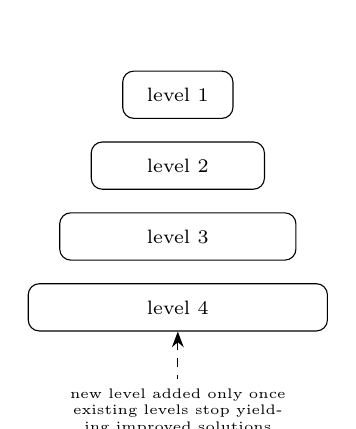
\begin{tikzpicture}[
        lvl/.style={draw, rounded corners, minimum height=6mm, font=\scriptsize, align=center},
    ]
        \node[lvl, minimum width=14mm] (l1) at (0,0)     {level 1};
        \node[lvl, minimum width=22mm] (l2) at (0,-9mm)  {level 2};
        \node[lvl, minimum width=30mm] (l3) at (0,-18mm) {level 3};
        \node[lvl, minimum width=38mm] (l4) at (0,-27mm) {level 4};
        \draw[{Stealth[length=2mm]}-, dashed] (l4.south) -- ++(0,-6mm)
            node[below, font=\tiny, align=center, text width=32mm]
            {new level added only once existing levels stop yielding improved solutions};
    \end{tikzpicture}
    \caption{P3's population pyramid: each level holds a population of growing size; a new level is added only
    when the levels below it stop producing improved solutions.}
    \Description{A vertical stack of four boxes labelled level 1 through level 4, growing wider from top to
    bottom, with an arrow noting that a new level is added only once existing levels stop yielding improved
    solutions.}
    \label{fig:p3-pyramid}
\end{figure}

\paragraph{Surrogate-assisted linkage learning.} CS-GOMEA pairs GOMEA with a convolutional surrogate on
synthetic combinatorial problems, and flags as open the surrogate's failure to use linkage information in its own
construction~\citep{dushatskiy2019csgomea}. Dushatskiy et al.\ integrate a surrogate with a P3 variant on an
ensemble-learning problem, where an SVR outperformed a neural
predictor~\citep{dushatskiy2021novelsurrogateassistedevolutionaryalgorithm}. LyMPuS integrates a surrogate
directly with linkage discovery and validates it with P3 on NK landscapes, Ising spin glasses, and
Max3Sat~\citep{przewozniczek2026lympus}; its empirical variant, eLyMPuS, discovers the dependency structure
incrementally rather than assuming it known. P3Net's surrogate follows eLyMPuS in being relative and
linkage-aware over an incompletely discovered structure, but regresses a continuous fitness difference rather
than making a discrete better/worse/ambiguous comparison, which places its mechanism closer to CS-GOMEA's and
forgoes eLyMPuS's monotonicity-conditional recovery guarantee.

\paragraph{Scale dependence.} The lineage's advantage over structure-blind search is documented to grow with
problem size. Goldman and Punch report a lower order of evaluation complexity for P3 than five competitors over
two orders of magnitude of problem size~\citep{goldman2015fast}; Qiao and Gallagher derive a GOMEA runtime bound
on concatenated traps whose gap over a $(1{+}1)$~EA widens with both subfunction count and
length~\citep{qiao2024gomearuntime}. Within NAS, den Ottelander et al.\ find MO-GOMEA, NSGA-II, local search, and
random search indistinguishable on NAS-Bench-101, while MO-GOMEA does beat random search on their larger MacroNAS
benchmarks~\citep{denottelander2021localsearch}.

\paragraph{Closest prior work.} Bartnik adapts SA-P3-GOMEA to multi-objective NAS on NAS-Bench-201, optimising
validation accuracy against measured GPU energy~\citep{bartnik2026evolutionary}. The surrogate is an absolute
regressor over the flat genotype (SVR, MLP, random forest, or gradient boosting); baselines are MO-LS and
surrogate-free MO-P3-GOMEA; the genotype is architecture-only. P3Net differs on all three axes: a relative,
linkage-aware surrogate; NSGA-II and NSGANetV2 as baselines; and a joint architecture-and-hyperparameter genotype,
to which, to our knowledge, no linkage-learning EA has previously been applied. Tran et al.\ also apply GOMEA to
NAS, but reduce cost through a training-free metric rather than a learned surrogate~\citep{tran2023gomeanas}.

\paragraph{LLM-based search.} Large language models enter the same search loop in three roles. As the optimiser
itself, GPT-4 proposes NAS-Bench-201 cells over ten iterations~\citep{zheng2023genius}, and a code-generating LLM
serves as the variation operator of a quality-diversity NAS~\citep{nasir2024llmatic}; outside NAS, LLM-driven
evolutionary search is competitive on the TSP only up to 20 nodes~\citep{liu2024lmea}, and LLMs underperform on
purely numerical black-box problems~\citep{huang2024llmblackbox}. As a surrogate, in-context LLM predictors match
conventional surrogates on 5- and 10-dimensional test functions at a higher inference
cost~\citep{hao2024llmsurrogate}, and an LLM performance predictor for machine-translation NAS attains the lowest absolute error but a
slightly weaker rank correlation than its baseline predictor~\citep{jawahar2024llmpp} -- ranking being what a
relative surrogate is used for. As a prior, LLMs warm-start or stand in for Bayesian
optimisation~\citep{liu2024llambo,zhang2024llmhpo} and prune a NAS search space by transferring design principles
from previously searched tasks~\citep{zhou2025lapt}. The documented gains concentrate in the early, sparse-data
phase~\citep{liu2024llambo}, on spaces of two to five hyperparameters and 10--30 evaluations in the main results of
Zhang et al.~\citep{zhang2024llmhpo}. Several studies trace them to prior knowledge rather than to feedback: LLMs
help Bayesian optimisation over molecules only when pretrained or fine-tuned on domain
data~\citep{kristiadi2024sober}, replacing observed outcomes with permuted labels leaves LLM-based experimental
design unaffected~\citep{gupta2025llmbo}, and within a fixed search space CMA-ES and TPE outperform LLM agents, a
hybrid of the two doing best~\citep{ferreira2026centaur}. Linkage learning is the opposite case: it uses no prior
and learns structure only from evaluations, with an advantage that grows with problem size (see
\emph{Scale dependence}). We found no direct comparison of the two families. We include no LLM-based arm, for
three reasons: it would draw on information outside the evaluation budget to which every other arm is held;
NAS-Bench-201 is public, and the GENIUS authors cannot rule out that GPT-4 has seen the benchmarks they
use~\citep{zheng2023genius}; and our question is why a linkage-learning engine fails to separate from random
search, which an added arm would not answer. The best-documented LLM role, warm-starting the sparse early phase,
nonetheless targets the uniform-random bootstrap that our diagnosis implicates (Section~\ref{sec:results}).

\paragraph{Joint NAS+HPO benchmarks and their limits.} JAHS-Bench-201 answers queries through a learned surrogate
over a mixed categorical/continuous joint space~\citep{bansal2022jahsbench}; NAS-HPO-Bench-II is a fixed lookup
table over architecture, learning rate, and batch size~\citep{hirose2021nashpobenchii}. Only the latter admits an
exactly enumerable oracle Pareto front, which we exploit for IGD+ (Section~\ref{sec:results}). Guerrero-Viu et
al.\ establish SH-EMOA and MO-BOHB as baselines for this joint setting~\citep{guerreroviu2021bagofbaselines}, none
of them a linkage-learning EA. Both benchmarks share the NAS-Bench-201 cell space~\citep{dong2020nasbench201} and
small-scale image classification. The benchmarking literature documents that search-space design accounts for
much of a method's reported performance and that rankings transfer poorly across
benchmarks~\citep{yang2020nasfrustratinglyhard,mehta2022nasbenchsuite}, that this particular cell space is
redundant and skewed toward already-good architectures~\citep{lopes2023nasbenchdesign}, and that conclusions
transfer inconsistently across task domains~\citep{tu2022nasbench360,duan2021transnasbench101}. Any result on
this family should be read against that.

\section{Problem Formulation}
\label{sec:problem-formulation}

\paragraph{Search space.} Let $[n] \triangleq \{1, \dots, n\}$. A genotype
$x = (x_1, \dots, x_n) \in \Lambda = \Lambda_1 \times \cdots \times \Lambda_n$ assigns one categorical value to
each coordinate. The first coordinates choose one operation per edge of the cell graph (e.g.\
\textsc{conv}$3{\times}3$, \textsc{skip}, \textsc{none}); the remaining coordinates choose training
hyperparameters such as learning rate or weight decay. Continuous hyperparameters are discretised into a fixed
grid before search (Section~\ref{sec:proposed-optimizer}), so $\Lambda$ is entirely categorical.

\paragraph{Validity.} A decoding function $D \colon \Lambda \to \mathcal{N}$ maps a genotype to a network. Not
every genotype decodes to a valid cell (e.g.\ no path from input to output). We write the constraint as
$g(x) \leq 0$ and the feasible set as $\Lambda^* = \{x \in \Lambda : g(x) \leq 0\}$.

\paragraph{Objectives.} Each $x \in \Lambda^*$ is assessed by
\begin{align}
    f_1(x) &= \text{validation error of } D(x) \quad \text{(minimised)}, \\
    f_2(x) &= \text{computational cost of } D(x) \quad \text{(minimised)}.
\end{align}
The cost measure is the one each benchmark exposes: model size in megabytes on JAHS-Bench-201, and tabulated
total training-and-validation time on NAS-HPO-Bench-II, which is read from the same lookup-table row as $f_1$
(one fixed recorded seed) and is therefore not cheaper to obtain. Both objectives are always queried at the highest fidelity $r_K$ the
benchmark tabulates. We seek the Pareto front
\[
    \mathcal{P}^* = \bigl\{ x \in \Lambda^* : \nexists\, x' \in \Lambda^*,\;
    \mathbf{f}(x') \preceq \mathbf{f}(x) \wedge \mathbf{f}(x') \neq \mathbf{f}(x) \bigr\},
\]
where $\mathbf{f} = (f_1, f_2)$ and $\preceq$ is component-wise $\leq$.

\paragraph{Budget.} The cost of search is the number of full evaluations of $\mathbf{f}$. Both benchmarks answer
deterministically, so each configuration is evaluated once; randomness across the $R$ independent runs of a
method comes from initialisation and stochastic operators, not from repeated queries.

\paragraph{Relative surrogate.} After $t$ full evaluations we hold
$\mathcal{H}_t = \{ (x^{(i)}, \mathbf{f}(x^{(i)})) \}_{i=1}^{t}$. Rather than regressing $f_1$ from an encoded
genotype, as NSGANetV2 does~\citep{lu2020nsganetv2}, P3Net's surrogate is \emph{relative} and
\emph{linkage-aware}. For a parent $x \in \Lambda^*$ and a candidate $x'$ that differs from $x$ only on a
linkage subset $F \subseteq [n]$ of the current dependency model ($x'_i = x_i$ for all $i \notin F$), it
predicts the effect of that local change,
\[
    \hat{\delta}_F(x, x') \approx f_1(x) - f_1(x'),
\]
trained on pairwise differences derived from $\mathcal{H}_t$. A positive $\hat\delta_F$ predicts an improvement.

\section{Proposed Optimizer}
\label{sec:proposed-optimizer}

\begin{figure*}[t]
    \centering
    \resizebox{\textwidth}{!}{%
    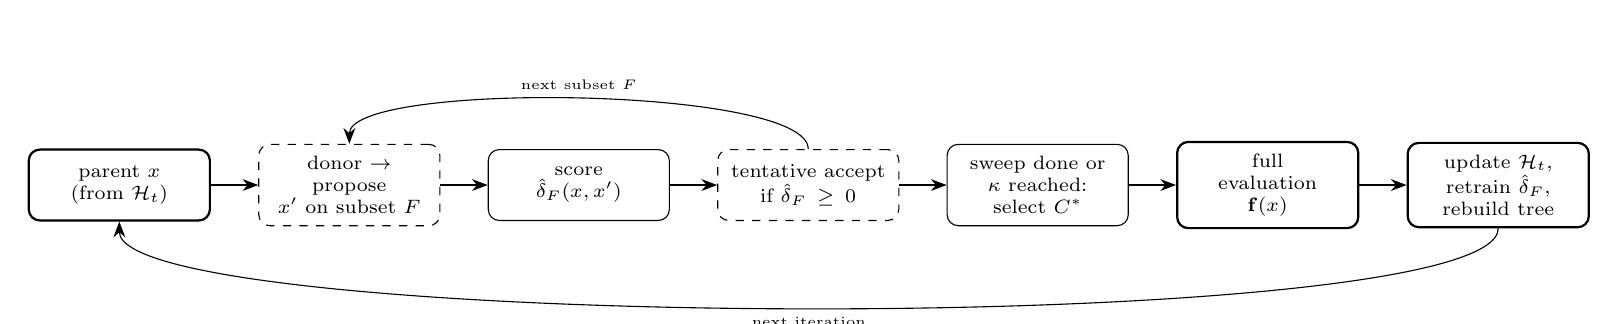
\begin{tikzpicture}[
        node distance=4mm and 6mm,
        box/.style={draw, rounded corners, align=center, font=\scriptsize, inner sep=1.5mm, minimum height=9mm, text width=20mm},
        real/.style={box, thick},
        tentative/.style={box, dashed},
        arr/.style={-{Stealth[length=2mm]}},
    ]
        \node[real]                       (parent) {parent $x$\\(from $\mathcal{H}_t$)};
        \node[tentative, right=of parent] (propose) {donor $\to$ propose\\$x'$ on subset $F$};
        \node[box, right=of propose]      (score) {score\\$\hat{\delta}_F(x,x')$};
        \node[tentative, right=of score]  (accept) {tentative accept\\if $\hat\delta_F \geq 0$};
        \node[box, right=of accept]       (select) {sweep done or\\$\kappa$ reached:\\select $C^*$};
        \node[real, right=of select]      (eval) {full\\evaluation\\$\mathbf{f}(x)$};
        \node[real, right=of eval]        (update) {update $\mathcal{H}_t$,\\retrain $\hat\delta_F$,\\rebuild tree};

        \draw[arr] (parent) -- (propose);
        \draw[arr] (propose) -- (score);
        \draw[arr] (score) -- (accept);
        \draw[arr] (accept) -- (select);
        \draw[arr] (select) -- (eval);
        \draw[arr] (eval) -- (update);

        \draw[arr] (accept.north) .. controls +(0,8mm) and +(0,8mm) .. (propose.north)
            node[midway, above, font=\tiny] {next subset $F$};

        \draw[arr] (update.south) .. controls +(0,-14mm) and +(0,-14mm) .. (parent.south)
            node[midway, below, font=\tiny] {next iteration};
    \end{tikzpicture}%
    }
    \caption{One P3Net iteration. Solid boxes hold fully evaluated individuals (members of $\mathcal{H}_t$);
    dashed boxes hold transient individuals accepted only by the surrogate. The upper loop repeats per linkage
    subset in the sweep, up to chain depth $\kappa$; the lower loop starts the next iteration.}
    \Description{A left-to-right flow diagram: parent x from H sub t leads to propose x-prime on subset F,
    then score via delta-hat sub F, then tentative accept if delta-hat is at least zero, then select C-star
    once the sweep is done or kappa is reached, then full evaluation, then update H sub t and rebuild the
    linkage tree. A small loop returns from tentative accept back to propose for the next subset, and a
    larger loop returns from the update step back to parent for the next iteration.}
    \label{fig:p3net-loop}
\end{figure*}

\paragraph{Representation and variation.} Following standard P3, a linkage tree is built by UPGMA-style
agglomerative clustering over a normalised mutual-information dependency measure between genotype
coordinates~\citep{goldman2014parameterless}. Each continuous hyperparameter is discretised once before search
into a fixed grid (e.g.\ log-spaced for learning rate), so the tree, its dependency measure, and optimal mixing
apply to the joint genotype unchanged. This trades hyperparameter resolution for keeping the comparison
attributable to engine and surrogate rather than to a new real-valued mixing operator; every baseline searches
the same discretised grid. As in the P3/GOMEA lineage there is no mutation: all variation comes from
linkage-guided optimal mixing against donors.

\paragraph{Surrogate.} $\hat\delta_F$ is a ridge regression (regularisation strength chosen by built-in
cross-validation) on the concatenated one-hot encodings of parent and candidate, with target
$f_1(x) - f_1(x')$. A linear model over this encoding can only represent
$w \cdot \mathrm{onehot}(x) - w \cdot \mathrm{onehot}(x')$: it is additive in the genotype coordinates and has
no term for how two jointly changed coordinates interact (Section~\ref{sec:results} examines the consequence).
An absolute estimate for a candidate reached by a chain $x_0, \dots, x_m$ of tentatively accepted modifications
from a fully evaluated ancestor $x_0$ is obtained by telescoping,
\[
    \hat{f}_1(x_m) = f_1(x_0) - \textstyle\sum_{i=1}^{m} \hat{\delta}_{F_i}(x_{i-1}, x_i).
\]

\paragraph{Search loop.} Each iteration (Figure~\ref{fig:p3net-loop}):
\begin{enumerate}
    \item For each parent, every linkage subset of the current tree is visited in random order; for each subset
    $F$ a donor proposes a modification restricted to $F$. Parents, donors, and the telescoping ancestor $x_0$
    are always drawn from $\mathcal{H}_t$, never from surrogate-only individuals.
    \item Each proposal $x'$ violating $g(x') \leq 0$ is discarded; the rest are scored by $\hat\delta_F$
    relative to the individual they modify.
    \item A proposal is tentatively accepted if $\hat\delta_F \geq 0$ and the sweep continues from it;
    otherwise it is rejected and the sweep moves to the next subset.
    \item Once a sweep completes, or $\kappa$ modifications have been accepted since the last full evaluation,
    the candidates nondominated in $(\hat f_1, f_2)$ among that iteration's outcomes form $C^*$. Restricting
    nondomination to one iteration keeps the compared estimates on a common surrogate snapshot.
    \item Each $x \in C^*$ is fully evaluated; duplicates already in $\mathcal{H}_t$ are served from a cache
    shared identically by every compared method and do not consume budget.
    \item $\mathcal{H}_t$ is updated, $\hat\delta_F$ refit, and the linkage tree rebuilt.
\end{enumerate}
$\kappa$ defaults to eLyMPuS's $2\lceil\log_2 n\rceil$~\citep{przewozniczek2026lympus}, used as a heuristic
bound on accumulated telescoping error rather than as a guarantee, since the monotonicity assumption behind that
bound is not expected to hold for network accuracy.

\paragraph{Population pyramid.} Following P3, the population is a sequence of levels of geometrically growing
target size, $2^k$ for level $k$. Two simplifications differ from canonical P3 and matter for
Section~\ref{sec:results}. First, only the newest level is swept, rather than cascading one individual's
improvement through every level. Second, a new level is grown as soon as a sweep over the current level fails to
increase that level's hypervolume against a padded nadir reference. A newly grown level is warm-started from the
nondominated front of $\mathcal{H}_t$, truncated to its target size by nondominated sorting and crowding distance
over $(\hat f_1, f_2)$, and filled the rest of the way by uniform random sampling. Levels that exceed their target
size are truncated by the same rule.

\section{Experiments}
\label{sec:results}

\subsection{Setup}

\paragraph{Benchmarks.} JAHS-Bench-201~\citep{bansal2022jahsbench} on all three of its built-in datasets
(CIFAR-10, Colorectal-Histology, Fashion-MNIST), and NAS-HPO-Bench-II~\citep{hirose2021nashpobenchii} within its
exhaustively tabulated 12-epoch range. The three JAHS-Bench-201 datasets test robustness within one benchmark
family, not generalisation beyond it.

\paragraph{Arms.} Table~\ref{tab:ablation-grid} organises the engine and surrogate ablations. NSGANetV2 is the
primary baseline; NSGA-Net and P3-alone are the surrogate-free versions of each engine; P3+abs.\ regressor
isolates the surrogate on P3Net's own engine. P3-alone originally used a population of 10 against 20 for every
other population-based arm, so two further arms, P3-alone-pop20 and P3-alone-pop40, remove that confound. Outside
the grid we compare against SH-EMOA~\citep{beume2007smsemoa} and MO-BOHB~\citep{falkner2018bohb}, established for
this joint setting~\citep{guerreroviu2021bagofbaselines}, and against TPE~\citep{bergstra2011tpe} and uniform
random search. The relative surrogate is defined only given a linkage tree, so an NSGA-II-plus-relative cell
cannot be built; the grid separates engine and surrogate as far as that permits. The surrogate ablation is
also not purely a change of formulation: P3Net's $\hat\delta_F$ uses ridge regression, while P3+abs.\ regressor
and NSGANetV2 use unregularised linear regression.

\begin{table}[t]
    \centering
    \caption{Engine/surrogate ablation grid. The NSGA-II/relative cell is not constructible. SH-EMOA, MO-BOHB,
    TPE, random search, and the two P3-alone population variants complete the eleven arms.}
    \label{tab:ablation-grid}
    \begin{tabular}{@{}lccc@{}}
        \toprule
         & \textbf{None} & \textbf{Absolute} & \textbf{Relative} $\hat{\delta}_F$ \\
        \midrule
        \textbf{NSGA-II} & NSGA-Net & NSGANetV2 & --- \\
        \textbf{P3}      & P3-alone & P3+abs.\ regressor & P3Net \\
        \bottomrule
    \end{tabular}
\end{table}

\paragraph{Fairness controls.} All arms share the genotype encoding, discretised hyperparameter grid, decoder,
validity check, full-evaluation budget, seed list, and deduplication cache. Discretising $\Theta$ equalises
resolution but is not neutral: it removes the real-valued crossover a native NSGANetV2 extension would use while
costing P3 nothing. A control arm running NSGANetV2 on continuous $\Theta$ was not completed, so this asymmetry is
acknowledged but not bounded. Budgets count full evaluations only; the surrogate arms additionally spend
wall-clock time on refitting and, for the P3 engine, on rebuilding the linkage tree, which we do not equalise.

\paragraph{Budgets and seeds.} Four tiers of $\{50, 100, 200, 350\}$ full evaluations. The second matches
JAHS-Bench-201's suggested protocol of about 100 evaluations~\citep{bansal2022jahsbench}; the largest matches the
full-evaluation count NSGANetV2 reports~\citep{lu2020nsganetv2}. All tiers are below NAS-HPO-Bench-II's
500-trial convention, deliberately, since the question concerns a limited budget. $R=30$ independent runs per
arm, per cell, with a fixed published seed list.

\paragraph{Metrics.} On NAS-HPO-Bench-II we enumerate all 196608 configurations, of which 188496 are valid,
and obtain the exact oracle Pareto front (25 points). We report IGD+ against it, with both objectives normalised
to the oracle front's range; across that front the training-time objective spans 18.53 times the range of the
error objective, so without normalisation it would dominate the distance. JAHS-Bench-201 admits no enumerable front, so we report hypervolume relative to a
best-known front: the nondominated set of every point evaluated by any arm, any budget, and any seed, pooled per
dataset. That front is computed once, persisted, and reused for every table, so adding an arm cannot retroactively
change the denominator of existing results.

\paragraph{Statistics.} P3Net is compared against each of the other ten arms, per (search space, budget) cell,
with paired Wilcoxon signed-rank tests, Holm--Bonferroni correction within the cell, and Cliff's $\delta$
reported for every comparison, following benchmarking practice for stochastic
optimisers~\citep{BartzBeielstein2020Benchmarking,Hansen2016b}. We orient $\delta$ so that a positive value
favours P3Net on both metrics.

\subsection{Headline comparison}

Tables~\ref{tab:heatmap-jahs}--\ref{tab:heatmap-nashpo} give Cliff's $\delta$ of P3Net against every other arm in
every cell; the supplementary material lists medians, IQRs, and corrected $p$-values.

% GENERATED by implementation/experiments/scripts/render_results_tex.py.
% Do not edit by hand -- regenerate from results/tables/ instead.

\begin{table}[t]
    \centering
    \footnotesize
    \caption{Effect-size heatmap, CIFAR-10: Cliff's $\delta$ of P3Net vs.\ each baseline on hypervolume relative to the frozen best-known front (higher is better). Blue favours P3Net, red favours the baseline; darker is larger $|\delta|$. Boxed cells reject $H_0$ at $\alpha=0.05$ (Holm--Bonferroni, per cell).}
    \label{tab:heatmap-jahs}
    \begin{tabular}{@{}lcccc@{}}
        \toprule
        \textbf{Method} & \textbf{50} & \textbf{100} & \textbf{200} & \textbf{350} \\
        \midrule
        P3-alone & \fcolorbox[HTML]{000000}{3987E5}{\makebox[2.4em]{\textcolor{white}{\textbf{+0.53}}}} & \fcolorbox[HTML]{000000}{184F95}{\makebox[2.4em]{\textcolor{white}{\textbf{+0.77}}}} & \fcolorbox[HTML]{000000}{184F95}{\makebox[2.4em]{\textcolor{white}{\textbf{+0.80}}}} & \fcolorbox[HTML]{000000}{86B6EF}{\makebox[2.4em]{\textcolor{black}{\textbf{+0.49}}}} \\
        P3-alone-pop20 & \colorbox[HTML]{86B6EF}{\makebox[2.4em]{\textcolor{black}{+0.36}}} & \fcolorbox[HTML]{000000}{3987E5}{\makebox[2.4em]{\textcolor{white}{\textbf{+0.55}}}} & \fcolorbox[HTML]{000000}{3987E5}{\makebox[2.4em]{\textcolor{white}{\textbf{+0.59}}}} & \fcolorbox[HTML]{000000}{3987E5}{\makebox[2.4em]{\textcolor{white}{\textbf{+0.58}}}} \\
        P3-alone-pop40 & \colorbox[HTML]{EAF2FC}{\makebox[2.4em]{\textcolor{black}{+0.05}}} & \fcolorbox[HTML]{000000}{86B6EF}{\makebox[2.4em]{\textcolor{black}{\textbf{+0.46}}}} & \fcolorbox[HTML]{000000}{86B6EF}{\makebox[2.4em]{\textcolor{black}{\textbf{+0.36}}}} & \colorbox[HTML]{CDE2FB}{\makebox[2.4em]{\textcolor{black}{+0.21}}} \\
        P3+abs.\ regressor & \colorbox[HTML]{EAF2FC}{\makebox[2.4em]{\textcolor{black}{+0.09}}} & \colorbox[HTML]{CDE2FB}{\makebox[2.4em]{\textcolor{black}{+0.14}}} & \colorbox[HTML]{CDE2FB}{\makebox[2.4em]{\textcolor{black}{+0.16}}} & \colorbox[HTML]{CDE2FB}{\makebox[2.4em]{\textcolor{black}{+0.17}}} \\
        \midrule
        NSGA-Net & \colorbox[HTML]{86B6EF}{\makebox[2.4em]{\textcolor{black}{+0.31}}} & \colorbox[HTML]{CDE2FB}{\makebox[2.4em]{\textcolor{black}{+0.29}}} & \colorbox[HTML]{F2A3A2}{\makebox[2.4em]{\textcolor{black}{-0.38}}} & \fcolorbox[HTML]{000000}{941F1F}{\makebox[2.4em]{\textcolor{white}{\textbf{-0.89}}}} \\
        NSGANetV2 & \colorbox[HTML]{EAF2FC}{\makebox[2.4em]{\textcolor{black}{+0.07}}} & \colorbox[HTML]{FDEEED}{\makebox[2.4em]{\textcolor{black}{-0.02}}} & \colorbox[HTML]{FBDCDB}{\makebox[2.4em]{\textcolor{black}{-0.26}}} & \colorbox[HTML]{F2A3A2}{\makebox[2.4em]{\textcolor{black}{-0.39}}} \\
        \midrule
        MO-BOHB & \colorbox[HTML]{FBDCDB}{\makebox[2.4em]{\textcolor{black}{-0.12}}} & \colorbox[HTML]{86B6EF}{\makebox[2.4em]{\textcolor{black}{+0.35}}} & \fcolorbox[HTML]{000000}{86B6EF}{\makebox[2.4em]{\textcolor{black}{\textbf{+0.46}}}} & \colorbox[HTML]{CDE2FB}{\makebox[2.4em]{\textcolor{black}{+0.28}}} \\
        random search & \colorbox[HTML]{EAF2FC}{\makebox[2.4em]{\textcolor{black}{+0.05}}} & \colorbox[HTML]{CDE2FB}{\makebox[2.4em]{\textcolor{black}{+0.12}}} & \colorbox[HTML]{CDE2FB}{\makebox[2.4em]{\textcolor{black}{+0.17}}} & \colorbox[HTML]{CDE2FB}{\makebox[2.4em]{\textcolor{black}{+0.25}}} \\
        SH-EMOA & \colorbox[HTML]{FBDCDB}{\makebox[2.4em]{\textcolor{black}{-0.17}}} & \fcolorbox[HTML]{000000}{F2A3A2}{\makebox[2.4em]{\textcolor{black}{\textbf{-0.49}}}} & \fcolorbox[HTML]{000000}{941F1F}{\makebox[2.4em]{\textcolor{white}{\textbf{-0.88}}}} & \fcolorbox[HTML]{000000}{941F1F}{\makebox[2.4em]{\textcolor{white}{\textbf{-0.96}}}} \\
        TPE & \colorbox[HTML]{FBDCDB}{\makebox[2.4em]{\textcolor{black}{-0.30}}} & \colorbox[HTML]{FBDCDB}{\makebox[2.4em]{\textcolor{black}{-0.28}}} & \fcolorbox[HTML]{000000}{E34948}{\makebox[2.4em]{\textcolor{white}{\textbf{-0.70}}}} & \fcolorbox[HTML]{000000}{941F1F}{\makebox[2.4em]{\textcolor{white}{\textbf{-0.82}}}} \\
        \bottomrule
    \end{tabular}
\end{table}

\begin{table}[t]
    \centering
    \footnotesize
    \caption{Effect-size heatmap, Colorectal-Histology: Cliff's $\delta$ of P3Net vs.\ each baseline on hypervolume relative to the frozen best-known front (higher is better). Blue favours P3Net, red favours the baseline; darker is larger $|\delta|$. Boxed cells reject $H_0$ at $\alpha=0.05$ (Holm--Bonferroni, per cell).}
    \label{tab:heatmap-colorectal}
    \begin{tabular}{@{}lcccc@{}}
        \toprule
        \textbf{Method} & \textbf{50} & \textbf{100} & \textbf{200} & \textbf{350} \\
        \midrule
        P3-alone & \fcolorbox[HTML]{000000}{3987E5}{\makebox[2.4em]{\textcolor{white}{\textbf{+0.67}}}} & \fcolorbox[HTML]{000000}{3987E5}{\makebox[2.4em]{\textcolor{white}{\textbf{+0.61}}}} & \fcolorbox[HTML]{000000}{86B6EF}{\makebox[2.4em]{\textcolor{black}{\textbf{+0.44}}}} & \colorbox[HTML]{FDEEED}{\makebox[2.4em]{\textcolor{black}{-0.04}}} \\
        P3-alone-pop20 & \fcolorbox[HTML]{000000}{86B6EF}{\makebox[2.4em]{\textcolor{black}{\textbf{+0.44}}}} & \colorbox[HTML]{86B6EF}{\makebox[2.4em]{\textcolor{black}{+0.32}}} & \colorbox[HTML]{FBDCDB}{\makebox[2.4em]{\textcolor{black}{-0.14}}} & \colorbox[HTML]{FBDCDB}{\makebox[2.4em]{\textcolor{black}{-0.18}}} \\
        P3-alone-pop40 & \colorbox[HTML]{EAF2FC}{\makebox[2.4em]{\textcolor{black}{+0.06}}} & \colorbox[HTML]{FDEEED}{\makebox[2.4em]{\textcolor{black}{+0.00}}} & \colorbox[HTML]{FBDCDB}{\makebox[2.4em]{\textcolor{black}{-0.30}}} & \fcolorbox[HTML]{000000}{E34948}{\makebox[2.4em]{\textcolor{white}{\textbf{-0.54}}}} \\
        P3+abs.\ regressor & \colorbox[HTML]{CDE2FB}{\makebox[2.4em]{\textcolor{black}{+0.27}}} & \colorbox[HTML]{EAF2FC}{\makebox[2.4em]{\textcolor{black}{+0.08}}} & \colorbox[HTML]{FBDCDB}{\makebox[2.4em]{\textcolor{black}{-0.12}}} & \colorbox[HTML]{FBDCDB}{\makebox[2.4em]{\textcolor{black}{-0.19}}} \\
        \midrule
        NSGA-Net & \colorbox[HTML]{CDE2FB}{\makebox[2.4em]{\textcolor{black}{+0.15}}} & \colorbox[HTML]{FDEEED}{\makebox[2.4em]{\textcolor{black}{-0.07}}} & \fcolorbox[HTML]{000000}{F2A3A2}{\makebox[2.4em]{\textcolor{black}{\textbf{-0.39}}}} & \fcolorbox[HTML]{000000}{941F1F}{\makebox[2.4em]{\textcolor{white}{\textbf{-0.82}}}} \\
        NSGANetV2 & \colorbox[HTML]{EAF2FC}{\makebox[2.4em]{\textcolor{black}{+0.08}}} & \fcolorbox[HTML]{000000}{F2A3A2}{\makebox[2.4em]{\textcolor{black}{\textbf{-0.48}}}} & \fcolorbox[HTML]{000000}{941F1F}{\makebox[2.4em]{\textcolor{white}{\textbf{-0.83}}}} & \fcolorbox[HTML]{000000}{941F1F}{\makebox[2.4em]{\textcolor{white}{\textbf{-0.81}}}} \\
        \midrule
        MO-BOHB & \colorbox[HTML]{CDE2FB}{\makebox[2.4em]{\textcolor{black}{+0.28}}} & \colorbox[HTML]{86B6EF}{\makebox[2.4em]{\textcolor{black}{+0.33}}} & \fcolorbox[HTML]{000000}{86B6EF}{\makebox[2.4em]{\textcolor{black}{\textbf{+0.49}}}} & \fcolorbox[HTML]{000000}{3987E5}{\makebox[2.4em]{\textcolor{white}{\textbf{+0.51}}}} \\
        random search & \colorbox[HTML]{EAF2FC}{\makebox[2.4em]{\textcolor{black}{+0.03}}} & \colorbox[HTML]{CDE2FB}{\makebox[2.4em]{\textcolor{black}{+0.20}}} & \colorbox[HTML]{CDE2FB}{\makebox[2.4em]{\textcolor{black}{+0.15}}} & \colorbox[HTML]{EAF2FC}{\makebox[2.4em]{\textcolor{black}{+0.08}}} \\
        SH-EMOA & \colorbox[HTML]{FDEEED}{\makebox[2.4em]{\textcolor{black}{-0.09}}} & \colorbox[HTML]{FBDCDB}{\makebox[2.4em]{\textcolor{black}{-0.28}}} & \fcolorbox[HTML]{000000}{941F1F}{\makebox[2.4em]{\textcolor{white}{\textbf{-0.80}}}} & \fcolorbox[HTML]{000000}{941F1F}{\makebox[2.4em]{\textcolor{white}{\textbf{-0.78}}}} \\
        TPE & \colorbox[HTML]{FBDCDB}{\makebox[2.4em]{\textcolor{black}{-0.20}}} & \colorbox[HTML]{FBDCDB}{\makebox[2.4em]{\textcolor{black}{-0.23}}} & \fcolorbox[HTML]{000000}{F2A3A2}{\makebox[2.4em]{\textcolor{black}{\textbf{-0.44}}}} & \fcolorbox[HTML]{000000}{F2A3A2}{\makebox[2.4em]{\textcolor{black}{\textbf{-0.45}}}} \\
        \bottomrule
    \end{tabular}
\end{table}

\begin{table}[t]
    \centering
    \footnotesize
    \caption{Effect-size heatmap, Fashion-MNIST: Cliff's $\delta$ of P3Net vs.\ each baseline on hypervolume relative to the frozen best-known front (higher is better). Blue favours P3Net, red favours the baseline; darker is larger $|\delta|$. Boxed cells reject $H_0$ at $\alpha=0.05$ (Holm--Bonferroni, per cell).}
    \label{tab:heatmap-fashion}
    \begin{tabular}{@{}lcccc@{}}
        \toprule
        \textbf{Method} & \textbf{50} & \textbf{100} & \textbf{200} & \textbf{350} \\
        \midrule
        P3-alone & \fcolorbox[HTML]{000000}{3987E5}{\makebox[2.4em]{\textcolor{white}{\textbf{+0.60}}}} & \fcolorbox[HTML]{000000}{184F95}{\makebox[2.4em]{\textcolor{white}{\textbf{+0.78}}}} & \fcolorbox[HTML]{000000}{184F95}{\makebox[2.4em]{\textcolor{white}{\textbf{+0.81}}}} & \fcolorbox[HTML]{000000}{184F95}{\makebox[2.4em]{\textcolor{white}{\textbf{+0.72}}}} \\
        P3-alone-pop20 & \fcolorbox[HTML]{000000}{86B6EF}{\makebox[2.4em]{\textcolor{black}{\textbf{+0.44}}}} & \fcolorbox[HTML]{000000}{3987E5}{\makebox[2.4em]{\textcolor{white}{\textbf{+0.62}}}} & \fcolorbox[HTML]{000000}{184F95}{\makebox[2.4em]{\textcolor{white}{\textbf{+0.74}}}} & \fcolorbox[HTML]{000000}{184F95}{\makebox[2.4em]{\textcolor{white}{\textbf{+0.77}}}} \\
        P3-alone-pop40 & \colorbox[HTML]{CDE2FB}{\makebox[2.4em]{\textcolor{black}{+0.22}}} & \fcolorbox[HTML]{000000}{86B6EF}{\makebox[2.4em]{\textcolor{black}{\textbf{+0.47}}}} & \fcolorbox[HTML]{000000}{3987E5}{\makebox[2.4em]{\textcolor{white}{\textbf{+0.62}}}} & \fcolorbox[HTML]{000000}{3987E5}{\makebox[2.4em]{\textcolor{white}{\textbf{+0.62}}}} \\
        P3+abs.\ regressor & \colorbox[HTML]{FDEEED}{\makebox[2.4em]{\textcolor{black}{-0.06}}} & \colorbox[HTML]{CDE2FB}{\makebox[2.4em]{\textcolor{black}{+0.19}}} & \colorbox[HTML]{CDE2FB}{\makebox[2.4em]{\textcolor{black}{+0.26}}} & \colorbox[HTML]{CDE2FB}{\makebox[2.4em]{\textcolor{black}{+0.27}}} \\
        \midrule
        NSGA-Net & \colorbox[HTML]{EAF2FC}{\makebox[2.4em]{\textcolor{black}{+0.10}}} & \colorbox[HTML]{CDE2FB}{\makebox[2.4em]{\textcolor{black}{+0.12}}} & \colorbox[HTML]{FDEEED}{\makebox[2.4em]{\textcolor{black}{-0.05}}} & \colorbox[HTML]{F2A3A2}{\makebox[2.4em]{\textcolor{black}{-0.36}}} \\
        NSGANetV2 & \colorbox[HTML]{CDE2FB}{\makebox[2.4em]{\textcolor{black}{+0.26}}} & \colorbox[HTML]{86B6EF}{\makebox[2.4em]{\textcolor{black}{+0.34}}} & \colorbox[HTML]{86B6EF}{\makebox[2.4em]{\textcolor{black}{+0.32}}} & \colorbox[HTML]{86B6EF}{\makebox[2.4em]{\textcolor{black}{+0.35}}} \\
        \midrule
        MO-BOHB & \colorbox[HTML]{86B6EF}{\makebox[2.4em]{\textcolor{black}{+0.39}}} & \fcolorbox[HTML]{000000}{86B6EF}{\makebox[2.4em]{\textcolor{black}{\textbf{+0.38}}}} & \colorbox[HTML]{CDE2FB}{\makebox[2.4em]{\textcolor{black}{+0.30}}} & \colorbox[HTML]{86B6EF}{\makebox[2.4em]{\textcolor{black}{+0.31}}} \\
        random search & \colorbox[HTML]{CDE2FB}{\makebox[2.4em]{\textcolor{black}{+0.14}}} & \colorbox[HTML]{CDE2FB}{\makebox[2.4em]{\textcolor{black}{+0.23}}} & \colorbox[HTML]{CDE2FB}{\makebox[2.4em]{\textcolor{black}{+0.22}}} & \colorbox[HTML]{CDE2FB}{\makebox[2.4em]{\textcolor{black}{+0.14}}} \\
        SH-EMOA & \colorbox[HTML]{FDEEED}{\makebox[2.4em]{\textcolor{black}{-0.02}}} & \colorbox[HTML]{FBDCDB}{\makebox[2.4em]{\textcolor{black}{-0.23}}} & \colorbox[HTML]{FBDCDB}{\makebox[2.4em]{\textcolor{black}{-0.23}}} & \fcolorbox[HTML]{000000}{E34948}{\makebox[2.4em]{\textcolor{white}{\textbf{-0.50}}}} \\
        TPE & \colorbox[HTML]{FDEEED}{\makebox[2.4em]{\textcolor{black}{-0.03}}} & \colorbox[HTML]{EAF2FC}{\makebox[2.4em]{\textcolor{black}{+0.06}}} & \colorbox[HTML]{FDEEED}{\makebox[2.4em]{\textcolor{black}{-0.06}}} & \colorbox[HTML]{EAF2FC}{\makebox[2.4em]{\textcolor{black}{+0.06}}} \\
        \bottomrule
    \end{tabular}
\end{table}

\begin{table}[t]
    \centering
    \footnotesize
    \caption{Effect-size heatmap, NAS-HPO-Bench-II: Cliff's $\delta$ of P3Net vs.\ each baseline on normalised IGD+ against the exact oracle front (lower is better). Blue favours P3Net, red favours the baseline; darker is larger $|\delta|$. Boxed cells reject $H_0$ at $\alpha=0.05$ (Holm--Bonferroni, per cell).}
    \label{tab:heatmap-nashpo}
    \begin{tabular}{@{}lcccc@{}}
        \toprule
        \textbf{Method} & \textbf{50} & \textbf{100} & \textbf{200} & \textbf{350} \\
        \midrule
        P3-alone & \colorbox[HTML]{EAF2FC}{\makebox[2.4em]{\textcolor{black}{+0.03}}} & \colorbox[HTML]{EAF2FC}{\makebox[2.4em]{\textcolor{black}{+0.08}}} & \colorbox[HTML]{EAF2FC}{\makebox[2.4em]{\textcolor{black}{+0.05}}} & \colorbox[HTML]{FBDCDB}{\makebox[2.4em]{\textcolor{black}{-0.19}}} \\
        P3-alone-pop20 & \colorbox[HTML]{FDEEED}{\makebox[2.4em]{\textcolor{black}{-0.00}}} & \colorbox[HTML]{EAF2FC}{\makebox[2.4em]{\textcolor{black}{+0.03}}} & \colorbox[HTML]{EAF2FC}{\makebox[2.4em]{\textcolor{black}{+0.03}}} & \colorbox[HTML]{EAF2FC}{\makebox[2.4em]{\textcolor{black}{+0.03}}} \\
        P3-alone-pop40 & \colorbox[HTML]{CDE2FB}{\makebox[2.4em]{\textcolor{black}{+0.14}}} & \colorbox[HTML]{EAF2FC}{\makebox[2.4em]{\textcolor{black}{+0.06}}} & \colorbox[HTML]{FBDCDB}{\makebox[2.4em]{\textcolor{black}{-0.11}}} & \colorbox[HTML]{FBDCDB}{\makebox[2.4em]{\textcolor{black}{-0.19}}} \\
        P3+abs.\ regressor & \colorbox[HTML]{CDE2FB}{\makebox[2.4em]{\textcolor{black}{+0.12}}} & \colorbox[HTML]{CDE2FB}{\makebox[2.4em]{\textcolor{black}{+0.10}}} & \colorbox[HTML]{CDE2FB}{\makebox[2.4em]{\textcolor{black}{+0.17}}} & \colorbox[HTML]{EAF2FC}{\makebox[2.4em]{\textcolor{black}{+0.07}}} \\
        \midrule
        NSGA-Net & \colorbox[HTML]{FDEEED}{\makebox[2.4em]{\textcolor{black}{-0.06}}} & \colorbox[HTML]{FBDCDB}{\makebox[2.4em]{\textcolor{black}{-0.19}}} & \fcolorbox[HTML]{000000}{941F1F}{\makebox[2.4em]{\textcolor{white}{\textbf{-0.72}}}} & \fcolorbox[HTML]{000000}{941F1F}{\makebox[2.4em]{\textcolor{white}{\textbf{-0.97}}}} \\
        NSGANetV2 & \colorbox[HTML]{FBDCDB}{\makebox[2.4em]{\textcolor{black}{-0.25}}} & \fcolorbox[HTML]{000000}{E34948}{\makebox[2.4em]{\textcolor{white}{\textbf{-0.52}}}} & \fcolorbox[HTML]{000000}{E34948}{\makebox[2.4em]{\textcolor{white}{\textbf{-0.65}}}} & \fcolorbox[HTML]{000000}{941F1F}{\makebox[2.4em]{\textcolor{white}{\textbf{-0.89}}}} \\
        \midrule
        MO-BOHB & \colorbox[HTML]{86B6EF}{\makebox[2.4em]{\textcolor{black}{+0.32}}} & \fcolorbox[HTML]{000000}{86B6EF}{\makebox[2.4em]{\textcolor{black}{\textbf{+0.42}}}} & \fcolorbox[HTML]{000000}{86B6EF}{\makebox[2.4em]{\textcolor{black}{\textbf{+0.46}}}} & \fcolorbox[HTML]{000000}{86B6EF}{\makebox[2.4em]{\textcolor{black}{\textbf{+0.41}}}} \\
        random search & \colorbox[HTML]{CDE2FB}{\makebox[2.4em]{\textcolor{black}{+0.17}}} & \colorbox[HTML]{CDE2FB}{\makebox[2.4em]{\textcolor{black}{+0.29}}} & \colorbox[HTML]{86B6EF}{\makebox[2.4em]{\textcolor{black}{+0.34}}} & \colorbox[HTML]{CDE2FB}{\makebox[2.4em]{\textcolor{black}{+0.19}}} \\
        SH-EMOA & \colorbox[HTML]{FBDCDB}{\makebox[2.4em]{\textcolor{black}{-0.28}}} & \fcolorbox[HTML]{000000}{E34948}{\makebox[2.4em]{\textcolor{white}{\textbf{-0.59}}}} & \fcolorbox[HTML]{000000}{941F1F}{\makebox[2.4em]{\textcolor{white}{\textbf{-0.92}}}} & \fcolorbox[HTML]{000000}{941F1F}{\makebox[2.4em]{\textcolor{white}{\textbf{-0.99}}}} \\
        TPE & \colorbox[HTML]{FBDCDB}{\makebox[2.4em]{\textcolor{black}{-0.18}}} & \fcolorbox[HTML]{000000}{E34948}{\makebox[2.4em]{\textcolor{white}{\textbf{-0.56}}}} & \fcolorbox[HTML]{000000}{941F1F}{\makebox[2.4em]{\textcolor{white}{\textbf{-0.76}}}} & \fcolorbox[HTML]{000000}{941F1F}{\makebox[2.4em]{\textcolor{white}{\textbf{-0.78}}}} \\
        \bottomrule
    \end{tabular}
\end{table}


% GENERATED by implementation/experiments/scripts/render_results_tex.py.
% Do not edit by hand -- regenerate from results/tables/ instead.

\textbf{59 of the 160 comparisons reject the null hypothesis} at $\alpha=0.05$. 28 favour the baseline over P3Net; 31 favour P3Net. The composition of each side matters more than the raw count. Of the 31 P3Net-favouring rejections, 24 are internal to the P3 engine's own surrogate-type/population comparisons (P3-alone, P3-alone-pop20, P3-alone-pop40, or P3+absolute-regressor) -- exactly the family the central question (Section~\ref{sec:introduction}) is staked on -- and seven are against a differently-engineered baseline (MO-BOHB, Colorectal-Histology, budget~350, $\delta=+0.511$, $p=0.009$; MO-BOHB, Colorectal-Histology, budget~200, $\delta=+0.491$, $p=0.014$; MO-BOHB, NAS-HPO-Bench-II, budget~200, $\delta=+0.458$, $p=0.004$; MO-BOHB, CIFAR-10, budget~200, $\delta=+0.456$, $p=0.009$). Of the 28 baseline-favouring rejections, 27 are losses to a differently-engineered method (SH-EMOA, TPE, NSGA-Net, or NSGANetV2) and one is a loss \emph{within} the P3-engine family itself -- cases where plain P3-alone, its population-size variants, or the absolute-regressor variant beats P3Net's own relative surrogate outright (P3-alone-pop40, Colorectal-Histology, budget~350, $\delta=-0.536$, $p=0.015$).

Significant losses to SH-EMOA, TPE, NSGA-Net, or NSGANetV2 grow with budget: none at budget~50, 5 at budget~100, 10 at budget~200, 12 at budget~350. Against NSGANetV2 specifically, P3Net loses significantly at every budget on Colorectal-Histology (from budget~100) and NAS-HPO-Bench-II (from budget~100), and does not separate at any budget on CIFAR-10 or Fashion-MNIST.

On Fashion-MNIST, P3Net significantly beats P3-alone at 4 of 4 budgets, P3-alone-pop20 at 4 of 4 budgets, P3-alone-pop40 at 3 of 4 budgets, with no ablation loss anywhere. On CIFAR-10, P3Net significantly beats P3-alone at 4 of 4 budgets, P3-alone-pop20 at 3 of 4 budgets, P3-alone-pop40 at 2 of 4 budgets, with no ablation loss anywhere. On Colorectal-Histology, P3Net beats P3-alone at 3 of 4 budgets, P3-alone-pop20 at 1 of 4 budgets, but loses to P3-alone-pop40 at budget~350 ($\delta=-0.536$). On NAS-HPO-Bench-II, no ablation comparison reaches significance in either direction.


All seven wins against a differently-engineered baseline are against MO-BOHB.

\paragraph{No separation from random search.} P3Net does not reject $H_0$ against uniform random search in any of
the sixteen cells (largest $|\delta|=0.336$). Repeating the identical protocol with random search as the
reference arm (Table~\ref{tab:vs-random}), P3+abs.\ regressor also separates in none, MO-BOHB in one, and every
other arm in at least six. The two arms that never separate are exactly the two that run P3Net's population
pyramid. P3Net's margin against each baseline tracks that baseline's own margin against random search almost
perfectly (Spearman $\rho=0.980$, $n=144$): across this grid, P3Net behaves as random search does.

\begin{table}[t]
    \centering
    \footnotesize
    \caption{Cells (of 16) in which each arm separates from uniform random search, same metric and per-cell
    correction as the headline comparison.}
    \label{tab:vs-random}
    \begin{tabular}{@{}lr@{\hspace{2em}}lr@{}}
        \toprule
        \textbf{Arm} & \textbf{Cells} & \textbf{Arm} & \textbf{Cells} \\
        \midrule
        SH-EMOA        & 13 & P3-alone-pop40      & 6 \\
        P3-alone       & 10 & TPE                 & 6 \\
        NSGANetV2      & 9  & MO-BOHB             & 1 \\
        NSGA-Net       & 8  & P3+abs.\ regressor  & 0 \\
        P3-alone-pop20 & 7  & \textbf{P3Net}      & \textbf{0} \\
        \bottomrule
    \end{tabular}
\end{table}

\begin{figure}[t]
    \centering
    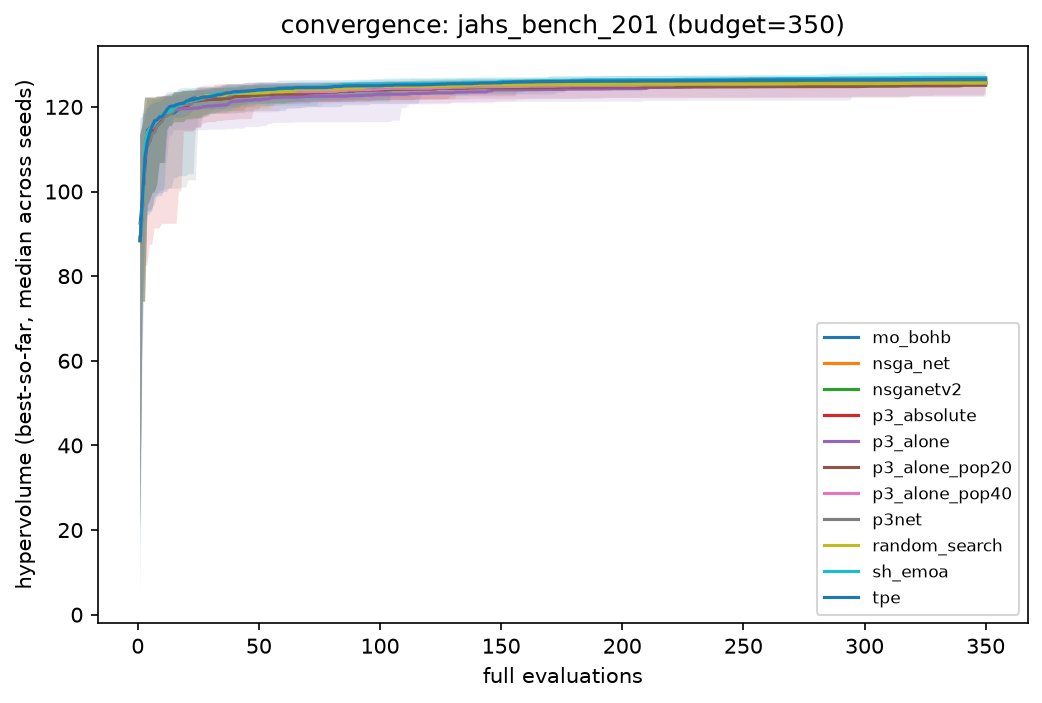
\includegraphics[width=\linewidth]{figures/convergence__jahs_bench_201__budget350.png}
    \caption{Median best-so-far relative hypervolume vs.\ full evaluations, all eleven arms, JAHS-Bench-201
    (CIFAR-10), budget~350. All arms reach a shared plateau within roughly the first tenth of the budget.}
    \label{fig:convergence-jahs-350}
\end{figure}

\subsection{Diagnosis}

\paragraph{The population pyramid spends the budget on random bootstrap.} Figure~\ref{fig:convergence-jahs-350}
shows every arm reaching a common plateau early, so the differences that matter are small and late. We therefore
measured what share of P3Net's proposals come from uniform-random level bootstrap rather than from
surrogate-guided mixing. Because level sizes grow geometrically, each new level is larger than all previous
levels combined, and filling it dominates the budget. The redesign described in
Section~\ref{sec:proposed-optimizer} -- warm-starting each new level from the current front and growing on a
hypervolume-contribution criterion rather than strict dominance -- was introduced in response to this, and all
reported numbers are from the grid re-run with it. Even so, the bootstrap share rises with budget on every search
space; on NAS-HPO-Bench-II it is 67.3\%, 77.6\%, 84.6\%, and 90.5\% at the four budgets, and at budget~350 it is
89.7\% (CIFAR-10), 91.7\% (Colorectal-Histology), 92.4\% (Fashion-MNIST), and 90.5\% (NAS-HPO-Bench-II). The
warm start does not change the growth rule itself, which is what forces the trend. This accounts directly for
the random-search-like behaviour above and for the pattern of losses widening with budget.

The evidence that this travels with the engine rather than with either surrogate is P3+abs.\ regressor. In an
earlier pass it ran on a flat, fixed-size population, and there it separated from random search in most cells.
Once rewritten to share P3Net's pyramid, it separates in none, and against P3Net itself it is indistinguishable
in all sixteen cells. With the engine confound removed, this grid shows no measurable advantage of the relative
surrogate over the absolute one. Conversely, the P3-alone arms use a fixed population and fail differently: they
stagnate on a small, repeatedly revisited set. Their median sweep count is 7--9 at budget~50 but 1508.5--2388.5
at budget~350, several times the budget itself, because most sweeps are served from the deduplication cache.
P3Net's wins over them are therefore at least partly broad random exploration beating a stalled narrow one, and
are not by themselves evidence for the relative surrogate.

\paragraph{The surrogate is additive and poorly calibrated.} The acceptance gate's precision -- the fraction of
surrogate-accepted modifications that turned out to improve -- is 0.498 over 14562 logged predictions:
indistinguishable from chance. It is highest while $|\mathcal{H}_t| \leq 30$ (0.551) and lower thereafter.
Magnitudes are worse than predicting the mean: $R^2$ between predicted and true $\delta$ is $-1.46$ (CIFAR-10),
$-2.08$ (Colorectal-Histology), $-3.28$ (Fashion-MNIST), and $-1.76$ (NAS-HPO-Bench-II). The error concentrates
at one pyramid level. At budget~350, predictions made while sweeping the level of size 16 have
$R^2=-4.71$ (MSE 766.7) against $R^2=+0.55$ (MSE 85.2) at size 2, roughly 9 times the error. That level is the
first whose sweep begins after a large, freshly bootstrapped population, when the linkage tree proposes subsets
for which few training pairs exist; this mechanism is plausible but not directly confirmed. Telescoping
accumulates error over the first steps of a chain (median squared error 26.5 at depth~1, 106.2 at depth~5) but
not monotonically beyond that.

Because $\hat\delta_F$ is linear in one-hot features, it cannot represent the joint effect of the coordinates
that linkage-guided crossover changes together, which is in tension with the premise of the crossover itself. As a
proxy for how much this matters per search space, we measure the out-of-sample $R^2$ gained by adding second-order
interaction terms touching at least one architecture edge to a main-effects model of $f_1$: $+0.016$ on
Fashion-MNIST, $+0.055$ on CIFAR-10, $+0.109$ on Colorectal-Histology, and $+0.259$ on NAS-HPO-Bench-II. This is
exactly the order in which P3Net's wins over its surrogate-free ablations weaken, from most complete on
Fashion-MNIST to none on NAS-HPO-Bench-II. The correspondence is observational; we did not intervene on it alone.
An arm that augments $\hat\delta_F$ with pairwise ``changed together'' interaction features, which fits a
constructed non-additive pattern that the plain model cannot represent, reaches significance against P3Net in 1
of 16 cells, in P3Net's favour. Added capacity did not translate into search performance.

\paragraph{Duplicate proposals are not what distinguishes P3Net.} Our initial hypothesis was that
dependency-aware variation would propose fewer duplicate genotypes. Mean proposal-time duplication is high for
the fixed-population P3 arms (P3-alone 0.734, P3-alone-pop20 0.448, P3-alone-pop40 0.187) and for SH-EMOA
(0.234), but P3Net (0.076) is not the lowest of the P3- and NSGA-II-engine arms: P3+abs.\ regressor (0.044),
NSGANetV2 (0.046), and NSGA-Net (0.038) all duplicate less. Whatever suppresses duplicates on the pyramid is not
specific to the relative surrogate.

\subsection{Isolation experiments}

The remaining candidate explanations are the joint genotype and the benchmark family. Both experiments below use
architecture-only NAS-Bench-201 through NATS-Bench~\citep{dong2021natsbench} ($n=6$ edge coordinates, no
$\Theta$), budgets 100 and 350, $R=30$, and the same statistical protocol; the best-known front is pooled within
this grid. Two deviations are forced by the benchmark interface: $f_2$ is FLOPs, as measured GPU
energy~\citep{bartnik2026evolutionary} is not a queryable field, and $f_1$ is test error. Because every arm is
scored identically, these deviations affect absolute values but not the comparison.

\begin{table}[t]
    \centering
    \footnotesize
    \caption{Architecture-only NAS-Bench-201. Relative hypervolume medians; Holm-corrected $p$ and Cliff's
    $\delta$ of the first arm against the second. No comparison rejects $H_0$.}
    \label{tab:isolation}
    \begin{tabular}{@{}llrrrr@{}}
        \toprule
        \textbf{Arm} & \textbf{vs.} & \textbf{Budget} & \textbf{Median} & \textbf{Adj.\ $p$} & \textbf{$\delta$} \\
        \midrule
        P3Net      & random search & 100 & 0.9851 & 0.9515 & $+0.016$ \\
        P3Net      & random search & 350 & 0.9923 & 0.7415 & $+0.118$ \\
        \midrule
        bartnik\_p3 & random search & 100 & 0.9856 & 1.0000 & $+0.113$ \\
        bartnik\_p3 & random search & 350 & 0.9935 & 0.5333 & $+0.273$ \\
        bartnik\_p3 & P3Net        & 100 & 0.9856 & 1.0000 & $+0.124$ \\
        bartnik\_p3 & P3Net        & 350 & 0.9935 & 0.9820 & $+0.222$ \\
        \bottomrule
    \end{tabular}
\end{table}

\paragraph{Removing the hyperparameter dimension.} Discretised hyperparameters enlarge $n$, and with it $\kappa$
and the space of linkage subsets, while plausibly carrying less combinatorial interaction than architecture edges.
If that diluted the linkage tree, removing $\Theta$ should help. It does not: P3Net still does not separate from
random search at either budget (Table~\ref{tab:isolation}), with both medians above 0.985.

\paragraph{The closest prior design.} Bartnik's SA-P3-GOMEA-class algorithm is documented to win on a search
space of this scale~\citep{bartnik2026evolutionary}. We reconstructed it as \texttt{bartnik\_p3}: canonical
single-individual-climbing P3, a random-forest absolute surrogate, and a quantile acceptance
gate~\citep{dushatskiy2021novelsurrogateassistedevolutionaryalgorithm}. This design avoids both of P3Net's
diagnosed defects: it has no geometrically bootstrapped levels, and its surrogate is not additive. On the
identical setup it does not separate from random search, nor from P3Net (Table~\ref{tab:isolation}). The null is
therefore not specific to P3Net's implementation; under this harness and baseline set, a design free of both
defects produces it as well.

\section{Conclusions}
\label{sec:conclusions}

\begin{itemize}
    \item P3Net combines P3's dependency modelling (a linkage tree built from pairwise mutual information over the genotype) with a relative surrogate that screens candidates before real evaluation, testing whether this combination improves surrogate-loop efficiency over NSGANetV2~\citep{lu2020nsganetv2} on a shared cell search space extended to joint architecture-and-hyperparameter NAS. The answer is no: P3Net does not separate from \texttt{random\_search} in any of the sixteen (search-space, budget) cells measured (Results), and its margin against every differently-engineered baseline correlates almost perfectly with that baseline's own margin against \texttt{random\_search} ($\rho=0.962$, $n=80$) -- indicating this comparison is dominated by a mechanism shared across arms, not a property specific to the relative surrogate. (The wider, ten-baseline version of this same correlation, run after the ablation family below was added to the grid, is reported further down.) The mechanistic account for this result is developed below.
    \item Limitations: surrogate quality plausibly depends on genotype encoding quality, though this dependency is not isolated by a dedicated ablation in the present design; the linkage tree is built from pairwise mutual information, which may be too coarse a signal to capture higher-order, deeply structured dependencies. JAHS-Bench-201 answers every query through a learned surrogate rather than measured data, so results on it inherit that surrogate's approximation error relative to real, independent training; since every compared method queries the same surrogate, systematic bias affects them equally, but this does not rule out the error correlating specifically with the structure P3Net exploits. A result that also holds on NAS-HPO-Bench-II, built from measured data, is therefore treated as the primary finding, and a result specific to JAHS-Bench-201 alone as requiring confirmation. NAS-HPO-Bench-II is inherently CIFAR-10-only; JAHS-Bench-201's single-dataset limitation raised by an earlier pass of this project (and shared with the closest prior work~\citep{bartnik2026evolutionary}, Related Work) is addressed by extending the grid to run across all three of JAHS-Bench-201's own built-in datasets (CIFAR-10, Colorectal-Histology, Fashion-MNIST) rather than only its CIFAR-10 default. This checks robustness across that benchmark's own dataset family rather than generalisation beyond it, and the honest result of that check is heterogeneity, not confirmation: the core surrogate-vs.-no-surrogate mechanism holds most completely on Fashion-MNIST, partially on CIFAR-10, and narrows on Colorectal-Histology (Results, ``Scope, and what would extend it''). NAS-HPO-Bench-II's own single-dataset ceiling still bounds what the measured-data leg of the comparison can speak to, and on that benchmark specifically the ablation result disappears and inverts at the highest budget tested. Results are further scoped to a single, shared architecture family (a NAS-Bench-201-style cell search space) and small-scale image classification across both benchmarks; neither a different architecture family nor a different task domain is tested here, and either would need different benchmark infrastructure entirely, not a configuration change. This specific limitation is not unique to the present comparison: the wider NAS benchmarking literature documents that both search-space design and task domain materially affect method rankings, and that conclusions drawn on one NAS benchmark frequently fail to transfer to another~\citep{yang2020nasfrustratinglyhard,mehta2022nasbenchsuite,lopes2023nasbenchdesign,tu2022nasbench360,duan2021transnasbench101} (Related Work).
    \item Future directions: stronger surrogate model (GNN over the cell graph), active learning to decide which candidates to evaluate fully, extension to architecture spaces with variable depth; training the surrogate on lower-fidelity observations $f_1^{(k)}$, $k<K$, rather than exclusively on full evaluations at $r_K$ as in the present work, using the fidelity ladder already introduced in Section~\ref{sec:problem-formulation}. This is left out here to keep the search loop's cost reduction cleanly attributable to the relative surrogate alone, but is a natural next lever once that attribution is established. Testing beyond this benchmark family's shared architecture family or task domain, or replacing benchmark-substrate evaluation with live training, would need substantially different infrastructure and is left as a separate undertaking. This is not merely a generic call for more testing: two specific observations from the present results motivate it directly (Results, ``Scope, and what would extend it''). The relative surrogate's measured advantage over the matched ablations, and the order-of-magnitude gap it opens in genotype duplication rate, both hold on a search space the wider NAS literature documents as comparatively small and unstructured~\citep{lopes2023nasbenchdesign}, while the P3/GOMEA lineage this work builds on has repeatedly shown that its advantage over generic search grows, rather than shrinks, as problem size and structural complexity increase~\citep{goldman2015fast,qiao2024gomearuntime,dushatskiy2019csgomea} (Related Work). That combination is a reasoned, evidence-based motivation for testing the same mechanism at larger scale or in a different task domain -- not a demonstration that it will succeed there, which only running that comparison could show. Extending to a new task domain is itself a precedented move in this literature, not a leap into the unknown: MoSegNAS carries the NSGANetV2~\citep{lu2020nsganetv2} lineage into semantic segmentation, but only after redesigning both the surrogate and the search space for the new task~\citep{lu2022mosegnas}, which is exactly why the present work treats a domain change, like live training, as a separate undertaking with its own infrastructure requirements rather than a configuration change on top of the present grid.
    \item A design-decision ablation round (Results, ``Design decisions: a P3Net ablation round'') resolves several open points empirically. Donor provenance and the population-truncation rule show no measurable effect across the full grid and are kept as designed. Computing $f_2$ fresh via the substrate's analytic cost hook, rather than inheriting it from the ancestor, gives a consistent, partly-significant hypervolume improvement and is adopted as the default -- though it also lowers acceptance-gate precision (Results, Surrogate quality); a follow-up investigation rules out a measurement artefact, accumulated chain error, a worse-fitting surrogate, and extrapolation distance as the cause without fully resolving why a lower-precision gate coexists with a better downstream result, left as a target for follow-up surrogate diagnostics. A simultaneous-cascade variant of the pyramid (every level swept every call, not only the newest) gives a similarly mixed, dataset-dependent result and a real per-iteration compute cost, and is not adopted.
    \item A later investigation into the per-dataset ranking pattern (Results, ``Diagnostics: population-pyramid bootstrap share'') identifies a more consequential mechanism: \texttt{Pyramid}'s geometric level growth, combined with starting every new level from an empty, uniform-randomly-bootstrapped population and sweeping only the newest level, structurally forces the uniform-random share of P3Net's own evaluation budget to rise with budget (measured $81.6\%\to93.0\%$ from budget~50 to~350 on NAS-HPO-Bench-II, cross-validated at $93$--$94\%$ across all four search spaces at budget~350). This share is large enough to explain why P3Net is not statistically distinguishable from \texttt{random\_search} in any of the sixteen cells measured, and why its margin against every differently-engineered baseline tracks that baseline's own margin against \texttt{random\_search} almost exactly ($\rho=0.962$, $n=80$): a substantial share of both the budget trend (widening losses to SH-EMOA/TPE/NSGA-Net/NSGANetV2) and the dataset trend (smallest losses on Fashion-MNIST, the search space where guided search barely beats uniform sampling at all) documented above is attributable to this pyramid-growth artefact rather than to a comparative property of the relative surrogate itself. A joint $\kappa$/acceptance-threshold sensitivity sweep (Results, ``Surrogate error accumulation'') rules out retuning either knob as a fix: the bootstrap-dominated share and fixed-budget hypervolume are both essentially flat across the full sensitivity grid.

    A redesign that warm-starts each newly grown level from $\mathcal{H}_t$'s current nondominated front,
rather than an empty population, and replaces the single-pass strict-Pareto-dominance stall trigger with a
hypervolume-contribution criterion, reduces the bootstrap-dominated share to $90$--$92\%$ across all four
search spaces at budget~350 (down from the $93$--$94\%$ documented above), confirmed on the full $R=30$ grid.
This is a real, directionally correct improvement, though a more modest one than the severity of the original
finding might suggest: the number of distinct levels grown by budget~350 is unchanged (7, sizes
$\{2,4,8,16,32,64,128\}$), meaning each level survives somewhat longer without meaningfully outpacing the
geometric progression's own growth rate. The consequence for the headline comparison: P3Net still does not
separate significantly from \texttt{random\_search} in any of the sixteen cells even under the fixed pyramid
($0/16$, Holm-corrected) -- the mechanism identified is real and the fix measurably shrinks it, but not by
enough, on this benchmark family and scale, to flip the headline finding. A further attempt -- starting each
level's real mixing much sooner, closer to how canonical P3~\citep{goldman2014parameterless} generates and
cascades one individual at a time rather than bootstrapping an entire level's target size with pure random
draws first -- causes a severe regression instead: this project's donor-pool-dependent optimal mixing, unlike
canonical P3's~\citep{goldman2014parameterless} single-individual hill climbing, degenerates without a real population to mix from. A
donor-pool-aware version of that same idea, not a hand-picked constant tuned against these four benchmarks
specifically, is left as the natural next candidate.
    \item A related but structurally independent limitation, surfaced alongside the pyramid finding above, concerns $\hat{\delta}_F$'s own model class rather than the search loop around it (Results, ``Diagnostics: surrogate representational capacity''): it, and the absolute regressor shared by the P3+absolute-regressor ablation and NSGANetV2~\citep{lu2020nsganetv2}, are all a plain \texttt{sklearn.LinearRegression} over one-hot genotype features, which can only represent additive, no-interaction fitness differences -- in tension with linkage-guided crossover's own premise that the variable groups it protects have a joint, not merely additive, effect on fitness (Related Work). A measured, dataset-ordered proxy for how much this misspecification actually costs (``architecture-involving epistasis'') tracks the same per-dataset pattern the pyramid finding above already partly explains, offered as a second, independently-motivated account rather than a competing one; which of the two, or what combination, is doing the explaining was not tested interventionally. Unlike P3Net's own linear surrogate, the two closest related methods sidestep this specific failure mode by construction -- Bartnik's~\citep{bartnik2026evolutionary} absolute regressor is fit as one of several nonlinear-capable model families, and eLyMPuS~\citep{przewozniczek2026lympus} is not a regression over a flat encoding at all -- making this a concrete, literature-motivated candidate for a follow-up alongside the pyramid redesign above, not a hypothetical one. A candidate fix, scoped to keep the relative/delta formulation's own data-efficiency advantage rather than swapping to a heavier model class, augments $\hat{\delta}_F$ with binary ``did coordinates $i$ and $j$ change together'' interaction columns, one per unordered coordinate pair, self-scoping to whichever linkage subset a given pair actually differs within without any separate bookkeeping. On a constructed non-additive pattern, unrepresentable by the original additive-only encoding by construction, the augmented surrogate fits it near-exactly -- direct evidence the added capacity is real. On the full $R=30$ grid as the new arm \texttt{p3net\_surrogate\_interactions}, the result is an honest null: against the Phase-2-fixed \texttt{p3net} baseline, significance is reached in $0/16$ cells, with small and sign-inconsistent effect sizes. The representational limit is real and measurably fixed, but this benchmark family's landscapes evidently do not carry enough exploitable interaction structure, at this scale, for the added capacity to change search outcomes -- consistent with the "not enough architectural complexity yet" account of P3Net's weak overall showing discussed above (Related Work).
    \item A third, complementary finding (Results, ``Surrogate quality: magnitude calibration'') concerns numerical stability rather than representational capacity or search-loop mechanics: $\hat{\delta}_F$'s predicted-delta \emph{magnitude} is calibrated far worse than trivially predicting the mean true delta in every search space, concentrated overwhelmingly in one specific pyramid level's first sweep pass immediately after its own bootstrap completes (a $6$--$19\times$ higher median squared error than any other level size, on real, repeated measurement). This is the textbook failure mode a point-estimate surrogate trusted without regard to its own reliability exhibits under a small, evolving training sample, for which the surrogate-assisted evolutionary computation literature's established remedy is regularisation or explicit uncertainty-aware model management~\citep{jin2011surrogate,hoerl1970ridge} -- distinct from, and adopted alongside, the pyramid-transition redesign above, since both concern exactly that same moment. Adopting \texttt{RidgeCV} as $\hat\delta_F$'s regressor does not correct it: on the full $R=30$ grid at budget~350, level~16 remains by far the worst-calibrated level ($R^2=-4.71$, MSE $766.7$) against every other level (best: level~2, $R^2=+0.55$, MSE $85.2$), a $\approx 9\times$ gap squarely inside the originally-documented $6$--$19\times$ range. Regularisation is the textbook remedy for unstable small-sample linear regression, but it does not, on this evidence, correct a systematic miscalibration concentrated at one specific, structurally-determined pyramid level -- the two problems this literature conflates (unstable coefficients vs.\ a landscape genuinely harder to model at that particular $|\mathcal{H}_t|$) may not be the same problem here, left as an open point for follow-up surrogate diagnostics rather than resolved by this pass.
    \item The P3+absolute-regressor ablation's own confound, noted above and in Results (``Diagnostics: surrogate representational capacity''), is closed by sharing P3Net's own \texttt{Pyramid} engine -- including the warm-start and hypervolume-contribution changes described above -- rather than a separate flat, fixed-size population, so this ablation isolates the surrogate alone, as the Baselines paragraph claims. On the full $R=30$ grid under the shared engine, the result is a null: P3Net vs.\ P3+absolute-regressor reaches significance in $0/16$ cells, in either direction. Once the population-engine confound that made the original comparison unfair is removed, this grid shows no measurable advantage of the relative surrogate over the absolute regressor -- a materially different, more cautious conclusion than the Baselines paragraph's original framing assumed, and one that should be read together with the other three null results just above: on this benchmark family and scale, none of the surrogate-side interventions tested in this pass (interaction features, RidgeCV, engine-sharing) separated from their respective baselines, even though each is independently, mechanistically confirmed to do what it was designed to do. The broader, every-arm-vs-\texttt{random\_search} check (Results, ``Diagnostics: population-pyramid bootstrap share'') updates accordingly: the overall reject rate drops from $67/160$ ($42\%$) pre-fix to $54/160$ ($34\%$) post-fix, and the cross-baseline-margin correlation stays essentially as strong ($\rho=0.945$, $n=144$, versus the pre-fix $\rho=0.962$) -- but the single largest mover in that table is P3+absolute-regressor itself, collapsing from $10/16$ significant wins over \texttt{random\_search} under its pre-fix flat population to $0/16$ once it shares P3Net's own bootstrap-dominated engine. That collapse is direct, mechanistic evidence for the account above: P3+absolute-regressor's apparent pre-fix strength was substantially an artefact of its \emph{different, non-Pyramid} population management, not of the absolute-regressor surrogate the ablation is meant to isolate -- the same pyramid-growth mechanism responsible for P3Net's own $0/16$ record, now shown to travel with the engine, not with either surrogate.
    \item \textbf{Why the results are what they are: a unified account, and an open, undertested hypothesis.} Four findings above are mechanistically independent but jointly consistent, and worth stating together rather than only as a list of separate diagnostics. (i)~\texttt{Pyramid}'s geometric growth structurally forces an ever-larger share of the budget into uniform-random bootstrap, a real and partially-fixed defect of the \emph{search engine}. (ii)~$\hat\delta_F$ is provably additive-only, a real and partially-fixed defect of the \emph{surrogate's model class}. (iii)~The benchmark family itself -- a NAS-Bench-201-style cell space -- is independently documented in the wider NAS literature as comparatively small, redundant, and unstructured, with most randomly sampled architectures already close to optimal~\citep{lopes2023nasbenchdesign}. None of (i)--(iii) alone fully explains the result: fixing (i) and (ii) each moved the needle measurably without flipping significance, exactly what a genuinely small-landscape ceiling on (iii) would predict regardless of how well (i) and (ii) are engineered around it. The P3/GOMEA lineage's own literature is consistent with this reading: its measured advantage over generic search grows, not shrinks, with problem size and structural complexity~\citep{goldman2015fast,qiao2024gomearuntime,dushatskiy2019csgomea} -- so a small-landscape ceiling is exactly the regime in which this family is expected to show the least of what it can do, independent of any implementation defect.

    A fourth candidate, distinct from (i)--(iii) and not yet disentangled from them, follows directly from the comparison to the closest prior work. Bartnik's SA-P3-GOMEA already demonstrates that a surrogate-assisted linkage learning algorithm \emph{can} win on a NAS-Bench-201-scale search space~\citep{bartnik2026evolutionary} -- an architecture-only one, with no hyperparameter dimension at all, using an absolute, nonlinear-capable regressor, and compared against MO-LS/MO-P3-GOMEA rather than NSGA-II/NSGANetV2. The present work differs from that success on all three axes simultaneously (surrogate formulation, baseline set, and, centrally, the joint architecture-and-hyperparameter genotype this work specifically contributes), so none of the results above can attribute the gap to any one of them in isolation. The joint-genotype axis is the one this work's own contribution rests on, and also the one never isolated: extending the genotype with discretised training hyperparameters ($\Theta$) grows $n$ and, with it, the chain-depth bound $\kappa=2\lceil\log_2(n)\rceil$ and the linkage tree's own search space of candidate subsets, but training hyperparameters such as learning rate or weight decay plausibly carry less multi-way, combinatorial epistasis than architectural edge choices do -- diluting, rather than enriching, the fraction of the linkage tree's sweep budget spent on subsets with real joint structure to exploit. This work's own measurements are consistent with, without confirming, that account: $98\%$ of real P3Net moves touch an architecture edge (Results, ``Diagnostics: surrogate representational capacity''), and the held-out ``architecture-involving epistasis'' proxy used there is defined specifically around architecture edges because that is where the signal concentrates -- both observations are compatible with $\Theta$ coordinates contributing comparatively little exploitable structure of the kind P3's linkage tree is built to find, though this was never tested by holding the joint-vs-architecture-only axis fixed while varying the others, and remains a hypothesis, not a finding. Section~\ref{sec:results}'s Scope discussion already treats testing at larger scale as the natural next step for (i)--(iii); isolating this fourth, joint-genotype-specific axis needs a different comparison -- P3Net run on an architecture-only search space directly comparable to Bartnik's~\citep{bartnik2026evolutionary} own, holding the surrogate and baseline set fixed.

    The isolating comparison motivated above was run as follows. \texttt{p3net} and \texttt{random\_search} were compared on architecture-only NAS-Bench-201 (no $\Theta$ at all, $n=6$ edge coordinates, $f_1=100-\text{test-accuracy}$, $f_2=\text{FLOPs}$ -- a documented deviation from Bartnik's~\citep{bartnik2026evolutionary} own measured GPU energy, which \texttt{nats\_bench}~\citep{dong2021natsbench} does not expose as a queryable field), holding the P3Net engine, surrogate, and baseline exactly as used throughout this work, at $R=30$ seeds and budgets $\{100,350\}$. The result does not support the fourth hypothesis: neither budget shows significance (adjusted $p=0.95$ at budget~$100$, $p=0.74$ at budget~$350$), and Cliff's delta is small and positive at both ($+0.02$, $+0.12$), with both methods' median relative hypervolume already at or above $0.985$. Removing the joint-genotype axis entirely -- the one candidate explanation this work's own contribution rests on -- leaves the headline result unchanged: P3Net still does not separate from random search, even on the exact class of search space where the closest prior work found separation. This shifts relative weight away from the fourth hypothesis and back toward (i)--(iii), particularly the benchmark family's own documented small-landscape ceiling~\citep{lopes2023nasbenchdesign}: both methods' near-ceiling medians on this run are consistent with a search space too easy, and too shallow in exploitable structure, for any of the search-side or surrogate-side differences among these methods to matter at this scale -- independent of whether the genotype carries a hyperparameter dimension or not.

    With the joint-genotype axis now ruled out, the remaining open explanations are the ones this account
    already narrows to: (iii) a benchmark family too small and unstructured for any tested method to separate
    from random search at this scale, and, within (i)--(ii), specific engineering choices this work's own
    \texttt{P3Net} makes differently from the two closest surrogate-assisted linkage-learning designs in the
    literature. Two concrete, direct tests follow, neither yet attempted here. First, testing (iii) properly
    means running on a larger or more structurally complex search space than any benchmark used in this
    work -- the step already motivated above (Results, ``Scope, and what would extend it''), now further
    supported by the isolation result: if the ceiling is the benchmark family itself, not the joint-genotype
    extension, then a bigger, deeper search space is the one lever left untried that this work's own diagnostics
    point to. Second, testing whether (i)--(ii) rather than (iii) are the operative bottleneck means holding this
    project's search space and evaluation infrastructure fixed while swapping in the two engines closest to
    \texttt{P3Net} in the literature it builds on: Bartnik's own \texttt{SA-P3-GOMEA}-class
    engine~\citep{bartnik2026evolutionary,dushatskiy2021novelsurrogateassistedevolutionaryalgorithm} (single-individual
    pyramid climb, nonlinear-capable absolute regressor) and Przewoźniczek et al.'s \texttt{eLyMPuS}/\texttt{OLyMPuS}
    family~\citep{przewozniczek2026lympus} (relative, non-monotonicity-based partial comparisons with guaranteed
    recursive linkage discovery, never previously evaluated on a NAS benchmark). If either reproduces this
    project's own null result on the same architecture-only search space, that is direct evidence for (iii);
    if either separates from random search where \texttt{P3Net} does not, that is direct evidence the gap sits in
    (i)--(ii), specifically in how \texttt{P3Net} instantiates them. Both comparisons are left as separate,
    dedicated undertakings rather than a configuration change on top of the present grid -- the second in
    particular requires generalising \texttt{eLyMPuS}'s binary-flip partial-comparison mechanism to NAS-Bench-201's
    five-valued categorical edges, which this work has not done and does not assume is straightforward.
\end{itemize}


\bibliographystyle{ACM-Reference-Format}
\bibliography{refs}

\clearpage
\onecolumn

\section*{Notes: Problem Formulation Design Log}

\emph{Working log, not part of the reviewed manuscript body: every architectural decision made while
formulating the problem, the surrogate, and the search engine, with the reasoning behind each choice and
where it lives in the text above.}

\subsubsection*{Problem representation}
\begin{longtable}{p{0.16\linewidth} p{0.28\linewidth} p{0.36\linewidth} p{0.13\linewidth}}
\toprule
\textbf{Decision} & \textbf{Specifics} & \textbf{Rationale / consequence} & \textbf{Location} \\
\midrule
\endhead
Architecture genotype & Vector $x=(x_1,\dots,x_n)\in\Lambda$, each $x_i$ from a finite set of operations on a cell-graph edge & Standard cell-based NAS encoding (as in NSGA-Net) & Problem Formulation \\
Joint-search extension & $\Lambda \to \Lambda_1\times\cdots\times\Lambda_n\times\Theta$, $\Theta\subset\mathbb{R}^m$ for training hyperparameters (LR, weight decay) & Answers Zela et al.: architecture and hyperparameters interact, so sequential tuning is unreliable & Problem Formulation \\
Scope of $\Theta$ & Training procedure only (LR, weight decay); structural capacity (cell count, channel width) stays part of the architecture / fidelity axes, not $\Theta$ & Matches the convention across the joint NAS+HPO literature (JAHS-Bench-201, NAS-HPO-Bench-II, Zela et al.) & Related Work \\
Handling $\Theta$'s continuity in P3 & \textbf{Discretisation} (option~i): each $\Theta$ coordinate is binned into a finite set before linkage learning; no separate mixing mechanism & Deliberate trade-off: lower HP-space resolution in exchange for a clean central question (does not conflate testing P3 with testing a novel continuous-mixing extension); RV-GOMEA-style mixing left as future work & Proposed Optimizer \\
Encoding in baselines & Same $\Theta$ discretisation imposed on NSGA-II/NSGANetV2 (rather than the unconstrained real-valued encoding a joint-setting extension of them would otherwise use); NSGANetV2 additionally run once more with that unconstrained real-valued encoding as a control & Discretisation is required for the ``identical genotype encoding'' fairness rule, but is not neutral: it costs NSGA-II/NSGANetV2 the real-valued crossover such an extension would otherwise use, while costing P3 nothing; the continuous-$\Theta$ control run bounds this asymmetry empirically instead of only asserting fairness by construction & Results, Fairness controls \\
\bottomrule
\end{longtable}

\subsubsection*{Decoding and validity}
\begin{longtable}{p{0.16\linewidth} p{0.28\linewidth} p{0.36\linewidth} p{0.13\linewidth}}
\toprule
\textbf{Decision} & \textbf{Specifics} & \textbf{Rationale / consequence} & \textbf{Location} \\
\midrule
\endhead
Decoding & $D:\Lambda\to\mathcal{N}$, maps a genotype to a network & --- & Problem Formulation \\
Validity & Constraint $g(x)\le 0$ (e.g.\ no input--output path); $\Lambda^*$ is the set of valid genotypes & Not every genotype decodes to a working network & Problem Formulation \\
Rejecting invalid candidates & $g(x)>0$ rejected before surrogate scoring & Saves surrogate evaluation cost & Proposed Optimizer \\
\bottomrule
\end{longtable}

\subsubsection*{What is being optimised}
\begin{longtable}{p{0.16\linewidth} p{0.28\linewidth} p{0.36\linewidth} p{0.13\linewidth}}
\toprule
\textbf{Decision} & \textbf{Specifics} & \textbf{Rationale / consequence} & \textbf{Location} \\
\midrule
\endhead
Objective 1 & $f_1(x)$ = validation error of $D(x)$, minimised & Standard predictive quality & Problem Formulation \\
Objective 2 & $f_2(x)=\phi(D(x))$ = computational cost (parameter count or FLOPs), computed analytically, minimised & Classic two-objective NAS formulation (quality vs.\ cost) & Problem Formulation \\
Resolution used for $f_2$ & Fixed at the highest fidelity level $r_K$'s setting, independent of the level at which $f_1$ happens to be queried & $f_2$ must not drift with fidelity level, so candidate costs stay comparable & Problem Formulation \\
Multi-objective formulation & Pareto front $\mathcal{P}^*$ --- standard dominance relation over $(f_1,f_2)$ & --- & Problem Formulation \\
\bottomrule
\end{longtable}

\subsubsection*{Budget and evaluation fidelity}
\begin{longtable}{p{0.16\linewidth} p{0.28\linewidth} p{0.36\linewidth} p{0.13\linewidth}}
\toprule
\textbf{Decision} & \textbf{Specifics} & \textbf{Rationale / consequence} & \textbf{Location} \\
\midrule
\endhead
Fidelity ladder & $r_1<\dots<r_K$, ordered by epoch count; if a benchmark exposes further resource axes (e.g.\ resolution), each level also fixes their value & Defined as general, substrate-level machinery (not tied to any one benchmark); full evaluation of $f_1$ is expensive, so a ladder is the natural vehicle for cheap filtering at lower fidelity, \emph{if} a method chooses to use one & Problem Formulation \\
P3Net's own fidelity scope & P3Net operates exclusively at full fidelity $r_K$; the ladder is \textbf{not} consumed by the search loop --- no candidate is ever scored via $f_1^{(k)}$, $k<K$; none of the Results baselines use it either & Keeps the search loop's cost reduction cleanly attributable to the relative surrogate alone, avoiding a third, unablated cost-reduction lever; kept as general infrastructure for a possible future multi-fidelity baseline (e.g.\ Hyperband-based), not an active component now; training on lower fidelities is noted as future work & Proposed Optimizer; Results; Conclusions \\
Noise handling & Stochastic substrates (live training, benchmark repeats): $s$ seeds, median used for selection/reporting; deterministic substrates (benchmark surrogate): no averaging. Both of P3Net's chosen benchmarks are deterministic, so $s=1$ throughout & Selection reliability under a non-deterministic objective, kept general for future stochastic substrates; $s$ (repeats of one query) is distinct from $R$ (independent search runs, Results) --- the two should not be conflated & Problem Formulation \\
Cost accounting & Counted exclusively in calls to $f_1$ (full evaluations), never in calls to $\hat{\delta}_F$ & Consistent with the paper's whole premise: full evaluation cost is the bottleneck & Problem Formulation \\
\bottomrule
\end{longtable}

\subsubsection*{Search engine}
\begin{longtable}{p{0.16\linewidth} p{0.28\linewidth} p{0.36\linewidth} p{0.13\linewidth}}
\toprule
\textbf{Decision} & \textbf{Specifics} & \textbf{Rationale / consequence} & \textbf{Location} \\
\midrule
\endhead
Algorithm & P3 instead of NSGA-II & Tests the hypothesis that dependency awareness beats crowding-distance selection under the same budget & Proposed Optimizer \\
Pyramid structure & P3 grows an ordered pyramid of populations of increasing size instead of a single fixed-size population, adding a level only once existing levels stop improving --- the ``parameter-less'' property & Explains why the name refers to a pyramid; canonically, promoting one solution up the pyramid costs a real evaluation per accepted local improvement, which is why the surrogate-free P3 ablation is expected to be budget-starved (see Baselines row below) & Related Work \\
Linkage tree & Agglomerative UPGMA clustering over normalised mutual information between genotype variables, standard P3 procedure, unmodified for the architecture part & Reuses a validated P3 mechanism unchanged & Proposed Optimizer \\
Tree rebuild granularity & Fixed for all sweeps within one iteration; rebuilt only at step~6, at iteration boundaries & Removes ambiguity about whether the tree could change mid-sweep --- it cannot & Proposed Optimizer \\
Crossover & Operates on variable groups (linkage subsets), not individual genes & Protects discovered groups of related design decisions from disruption & Proposed Optimizer \\
No mutation operator & All variation comes from the crossover-guided optimal-mixing sweep; no separate mutation step & Inherited from the P3/GOMEA lineage; diversity relies entirely on recombination against the linkage tree, not random perturbation & Proposed Optimizer \\
\bottomrule
\end{longtable}

\subsubsection*{Surrogate}
\begin{longtable}{p{0.16\linewidth} p{0.28\linewidth} p{0.36\linewidth} p{0.13\linewidth}}
\toprule
\textbf{Decision} & \textbf{Specifics} & \textbf{Rationale / consequence} & \textbf{Location} \\
\midrule
\endhead
Surrogate type & \textbf{Relative and linkage aware}: $\hat{\delta}_F(x,x')\approx f_1(x)-f_1(x')$ for a pair differing only on subset $F$, instead of absolute regression from the full encoding (as in NSGANetV2) & This is the property that separates P3Net from NSGANetV2 already at the problem-formulation level & Problem Formulation \\
Mechanism lineage & Mechanistically closer to CS-GOMEA (regression on continuous fitness differences, no formal guarantee); philosophically closer to eLyMPuS (relative estimator over an incompletely discovered dependency structure, not assumed known in advance) & NAS validation accuracy does not decompose into subfunctions (no gray-box access); P3Net accordingly forgoes eLyMPuS's monotonicity-conditional recovery guarantee & Related Work; Proposed Optimizer \\
Reconstructing an absolute estimate & Telescoping along the chain of accepted modifications back to the nearest fully-evaluated ancestor: $\hat f_1(x_m)=f_1(x_0)-\sum_i\hat\delta_{F_i}$ & Scores a candidate deep in the sweep without a full evaluation at every step & Proposed Optimizer \\
Ancestor guarantee & $x_0$ is always drawn from $\mathcal{H}_t$ (completed steps 5--6), never a surrogate-only individual mid-sweep & Closes a gap where the telescoping construction could otherwise bottom out on an unknown $f_1(x_0)$ & Proposed Optimizer \\
Donor provenance (open) & Whether the donor drawn in step~1 must also come from $\mathcal{H}_t$, like the parent and $x_0$, or may be a transient surrogate-only individual, is not yet stated & Flagged as TODO in text; parents and $x_0$ already carry this restriction, the donor does not yet & Proposed Optimizer \\
Surrogate training & On pairwise differences drawn from $\mathcal{H}_t$ (the set of full evaluations so far) & --- & Problem Formulation \\
Refresh cycle & $\mathcal{H}_t$, $\hat\delta_F$, and the linkage tree are rebuilt after every round of full evaluations & Surrogate and dependency structure co-evolve with the population & Proposed Optimizer \\
\bottomrule
\end{longtable}

\subsubsection*{Search loop}
\begin{longtable}{p{0.06\linewidth} p{0.79\linewidth} p{0.10\linewidth}}
\toprule
\textbf{Step} & \textbf{What happens} & \textbf{Location} \\
\midrule
\endhead
1 & P3 generates candidates through a full optimal-mixing sweep along the linkage tree & Proposed Optimizer \\
2 & Every proposal is scored relative to its immediate predecessor in the sweep, via $\hat\delta_F$ & Proposed Optimizer \\
3 & Tentative acceptance if the surrogate predicts non-negative improvement (zero threshold by default, swept in Results); otherwise rejection and move to the next subset & Proposed Optimizer \\
4 & Once the sweep completes (or is cut short by $\kappa$), $C^*$ is selected as the candidates nondominated in $(\hat f_1, f_2)$ & Proposed Optimizer \\
5 & Full evaluation of every $x\in C^*$ & Proposed Optimizer \\
6 & Update $\mathcal{H}_t$, retrain $\hat\delta_F$, rebuild the linkage tree & Proposed Optimizer \\
\bottomrule
\end{longtable}

\subsubsection*{Safeguards and auxiliary parameters}
\begin{longtable}{p{0.16\linewidth} p{0.28\linewidth} p{0.36\linewidth} p{0.13\linewidth}}
\toprule
\textbf{Decision} & \textbf{Specifics} & \textbf{Rationale / consequence} & \textbf{Location} \\
\midrule
\endhead
Deduplication & Candidates already present in $\mathcal{H}_t$ skip re-evaluation; applied identically to every compared method as part of the shared evaluation harness, not just within P3Net's loop & Direct response to the genotype-to-phenotype redundancy documented in NSGA-Net; uniform application prevents the saving from inflating P3Net's apparent efficiency relative to baselines that could equally use it & Proposed Optimizer; Results, Fairness controls \\
Chain depth $\kappa$ & Maximum number of tentatively accepted modifications before a full evaluation is forced & Bounds the accumulation of surrogate error along a sweep & Proposed Optimizer \\
Acceptance threshold & Step-3 acceptance rule uses a zero threshold by default ($\hat\delta_F \geq 0$) & Simplest heuristic consistent with standard optimal-mixing acceptance (no worsening); swept jointly with $\kappa$ rather than assumed adequate & Proposed Optimizer; Results \\
Default value of $\kappa$ & Initialised at eLyMPuS's $2\lceil\log_2 n\rceil$-step bound, where $n$ is the dimensionality of the full extended, discretised genotype (architecture + $\Theta$), not the architecture-only count of Problem Formulation --- as a heuristic, \emph{not} a derivation from the monotonicity guarantee that bound relies on (which does not hold here) & Honest acknowledgement that the theoretical guarantee does not transfer to NAS; sensitivity tested empirically, jointly with the acceptance threshold above & Proposed Optimizer; Results \\
Full sweep, not single modification & Candidate generation always runs the complete optimal-mixing sweep & Consistency with the variation operator P3's own guarantees rely on & Proposed Optimizer \\
No guarantee for $\hat\delta_F$ & Treated as a learned heuristic estimator, without eLyMPuS's recovery guarantee (monotonicity assumption broken for NN fitness) & Scientific caution --- does not import a theoretical guarantee into a domain where it does not hold & Proposed Optimizer \\
Nondomination reference frame & Step~4 compares only candidates from the same search iteration (same $\mathcal{H}_t$ snapshot) & Prevents mixing $\hat f_1$ estimates against a drifting surrogate across iterations & Proposed Optimizer \\
\bottomrule
\end{longtable}

\subsubsection*{Benchmarks and experimental scope}
\begin{longtable}{p{0.16\linewidth} p{0.28\linewidth} p{0.36\linewidth} p{0.13\linewidth}}
\toprule
\textbf{Decision} & \textbf{Specifics} & \textbf{Rationale / consequence} & \textbf{Location} \\
\midrule
\endhead
Primary benchmarks & JAHS-Bench-201 (Category~2 --- continuous surrogate, no enumerable oracle) and NAS-HPO-Bench-II (Category~1 --- discrete grid, exact oracle) --- both, deliberately, side by side & Deterministic objective, computable oracle front, bounded evaluation budget; a result holding on both is reported as primary, on one as benchmark-specific & Related Work; Results \\
Baselines & NSGANetV2 (primary, discretised $\Theta$); NSGANetV2 extended to the joint setting with an unconstrained, real-valued $\Theta$ (control, isolating the effect of discretisation itself); NSGA-Net with no surrogate, every candidate fully evaluated (engine-only ablation, NSGA-II side, symmetric to the P3 row below); P3 without a surrogate (engine-only ablation, P3 side); P3 with an absolute regressor in the NSGANetV2 style (surrogate-only ablation); SH-EMOA and MO-BOHB, the baselines established for this exact joint setting on these same two benchmarks~\citep{guerreroviu2021bagofbaselines}; random search and TPE (sanity checks) & Attributes gains to search engine vs.\ surrogate vs.\ discretisation as far as the design permits; not a full orthogonal factorial, since the relative surrogate $\hat\delta_F$ is only defined given a linkage tree, so an NSGA-II-plus-relative-surrogate cell does not exist. SH-EMOA/MO-BOHB added because, unlike NSGANetV2, they were never imported from an architecture-only setting and require no such extension & Results \\
P3-without-surrogate budget reality & Follows the canonical optimal-mixing acceptance rule: every accepted step within a sweep is gated by a \emph{real} $f_1$ evaluation, as in P3's own hill-climbing/cross-level mixing & Expected to exhaust most or all of a 50--200 budget within very few sweeps; reported explicitly (number of full sweeps completed within budget) so a weak result reads as budget starvation, not engine failure --- this collapse is itself informative, motivating the surrogate & Results, Baselines \\
Full evaluation budget tiers & Three tiers, $\{50, 100, 200\}$ full evaluations, doubling at each step; $R=10$ independent seeds & Verified against three literature-specific figures, not chosen arbitrarily: (1) JAHS-Bench-201's own suggested protocol is $\approx$100 evaluations, min.\ 10 seeds~\citep{bansal2022jahsbench} -- matches the middle tier and $R$ directly; (2) NSGANetV2 itself uses exactly 350 full evaluations (Table 2) to reach its reported results~\citep{lu2020nsganetv2} -- the top tier (200) stays below this; (3) NAS-HPO-Bench-II's own paper benchmarks search algorithms at 500 trials~\citep{hirose2021nashpobenchii} -- all three tiers stay below this too, deliberately, since the central question is about a \emph{limited} budget (Introduction) & Results \\
Metrics & Fixed-budget hypervolume always; IGD+ only where the oracle front is enumerable (i.e.\ NAS-HPO-Bench-II only), otherwise hypervolume relative to a best-known front (open: precise definition, e.g.\ union of all points evaluated by any compared method, still TODO) & Metric matched to what each benchmark actually offers & Results \\
Statistical plan & Paired Wilcoxon signed-rank test, Holm--Bonferroni correction, effect size (e.g.\ Cliff's delta) reported with every corrected $p$-value & Deliberately stricter than the uncorrected comparisons in Bartnik & Results \\
Comparison set for correction & P3Net vs.\ each of the other nine arms, per benchmark and per budget tier --- not every pairwise combination among all arms & Makes explicit what Holm--Bonferroni is correcting across, since the corrected significance threshold depends on this count & Results, Statistical plan \\
Diagnostics & Genotype duplication rate and archive turnover, measured under identical genotype encoding \emph{and} an identically applied deduplication cache across methods; counted at proposal time, not evaluation time & Empirically tests whether the NSGA-Net-derived motivation (duplication redundancy) actually transfers to the joint arch+HP genotype, apples-to-apples across methods, without the comparison being confounded by asymmetric caching or by measurement point & Results \\
Reproducibility & Cache keyed by genotype, experiment type, and a protocol version string & Automatic invalidation of stale cache entries on any settings change & Results \\
\bottomrule
\end{longtable}

\subsubsection*{Scope boundaries (deliberately excluded / distinguished)}
\begin{longtable}{p{0.20\linewidth} p{0.62\linewidth} p{0.13\linewidth}}
\toprule
\textbf{Decision} & \textbf{Specifics} & \textbf{Location} \\
\midrule
\endhead
Gray-box vs.\ black-box & P3Net operates in the black-box regime (NAS accuracy is not decomposable); explicitly distinguished from the gray-box optimisation of Whitley/Chicano/Goldman used in the GOMEA line & Related Work \\
Benchmark surrogate vs.\ search-time surrogate & JAHS-Bench-201's surrogate stands in for the objective once, offline, before search begins; P3Net's surrogate is fitted incrementally during search --- two independent design choices & Related Work \\
Delta vs.\ closest prior work (Bartnik) & Bartnik: absolute regressor, MO-LS/MO-P3-GOMEA baselines (not NSGA-II/NSGANetV2), architecture-only search (NAS-Bench-201, no $\Theta$) --- P3Net differs on all three axes at once & Related Work \\
\bottomrule
\end{longtable}

\subsubsection*{Settled review decisions (do not re-open without new information)}
\emph{Before flagging an issue in a new review pass, check this table first. ``Fixed'' items have already
been addressed in the text at the cited location. ``Rejected'' items were considered and deliberately left
unchanged -- re-raising them as if undiscovered is not useful without a concrete reason the rejection no
longer holds. This table itself is exempt from review, per the standard reviewer instructions.}
\begin{longtable}{p{0.24\linewidth} p{0.08\linewidth} p{0.55\linewidth} p{0.09\linewidth}}
\toprule
\textbf{Item} & \textbf{Status} & \textbf{Resolution / reason} & \textbf{Where} \\
\midrule
\endhead
Related Work placed after Proposed Optimizer & Rejected & Author's explicit choice, confirmed after review; forward references (eLyMPuS, GOMEA lineage) are glossed inline at first use instead of reordering sections & Introduction; Proposed Optimizer \\
Deduplication cache scope & Fixed & Applies identically to every compared method as shared harness, not only P3Net & Proposed Optimizer; Results \\
Discretisation asymmetry (NSGA-II loses native crossover, P3 does not) & Fixed & Bounded empirically via a native-continuous-$\Theta$ NSGANetV2 control baseline, not just acknowledged & Results, Baselines/Fairness controls \\
Engine$\times$surrogate ablation not a full factorial & Fixed & Stated explicitly: relative surrogate needs a linkage tree, so an NSGA-II+relative-surrogate cell cannot exist & Results, Baselines \\
$\mathcal{H}_t$ vs.\ $D$ notational collision & Fixed & Observation dataset renamed $\mathcal{H}_t$ throughout & Problem Formulation; Proposed Optimizer; Results \\
Multi-fidelity ladder apparatus vs.\ unused in practice & Fixed & Stated explicitly that no current baseline exploits it; kept as general infrastructure for a possible future multi-fidelity baseline & Problem Formulation \\
Full evaluation budget tiers unsourced & Fixed & $\{50,100,200\}$, $R=10$, each anchored to a verified literature figure (JAHS-Bench-201 protocol, NSGANetV2's 350, NAS-HPO-Bench-II's 500) & Results, Budgets \\
``P3 alone'' ablation: acceptance mechanism and budget feasibility undefined & Fixed & Canonical optimal-mixing acceptance (real $f_1$ gates every accepted step) stated explicitly; expected budget starvation stated as an informative result, not hidden; sweeps-completed-within-budget reported as a diagnostic & Results, Baselines \\
Missing NSGA-II-side engine-only baseline (asymmetric with ``P3 alone'') & Fixed & Added: NSGA-Net (no surrogate, full training every candidate) as the symmetric engine-only ablation & Results, Baselines \\
$s$ (evaluation-noise seeds) vs.\ $R$ (independent runs) terminology collision & Fixed & Distinguished explicitly; both chosen benchmarks are deterministic, so $s=1$ throughout & Problem Formulation \\
$\kappa$'s default bound: does $n$ include $\Theta$? & Fixed & Clarified: $n$ is the full extended, discretised genotype dimensionality & Proposed Optimizer \\
Telescoping construction: is the ancestor $x_0$ guaranteed fully evaluated? & Fixed & Stated explicitly: parents and $x_0$ are always drawn from $\mathcal{H}_t$, never surrogate-only individuals & Proposed Optimizer \\
Linkage tree rebuild granularity (within a sweep vs.\ between rounds) & Fixed & Stated explicitly: fixed within an iteration, rebuilt only at step~6 & Proposed Optimizer \\
Statistical plan: ``full set of comparisons'' undefined & Fixed & Enumerated: P3Net vs.\ each of the other nine arms, per benchmark and budget tier & Results, Statistical plan \\
Diagnostics: duplication rate measured pre- or post-dedup-cache? & Fixed & Stated explicitly: counted at proposal time, not evaluation time & Results, Diagnostics \\
P3 pyramid / ``parameter-less'' never explained & Fixed & One paragraph added at first substantive mention of P3 & Related Work \\
NSGANetV2's ``few hundred'' evaluations left vague while Results cites 350 & Fixed & Related Work now states the precise figure (350) at first mention & Related Work \\
Budget-tier justification citing benchmark-mismatch as a reason for the dual-benchmark design & Fixed & Circular clause removed; the dual-benchmark choice is justified once, in Related Work (Category~1/2), not re-derived from budget numbers & Results, Budgets \\
``in the spirit of eLyMPuS'' phrase repeated across three sections & Fixed (superseded) & No longer applies: the Proposed Optimizer instance was replaced by the CS-GOMEA/eLyMPuS mechanism-vs-philosophy split above, so the phrase now appears once, in Introduction, as a forward-reference gloss & Introduction \\
Three-surveys citation appearing twice in Related Work & Rejected & Not a duplication: the two passages draw two distinct claims (dominant paradigm; absence of linkage learning as a category) from the same three surveys & Related Work \\
No explicit directional hypothesis (H1) & Rejected & Kept as a neutral research question by deliberate choice; GECCO framing convention, not a defect & Introduction \\
Results register (``must not allow'' imperative phrasing) & Deferred & Results is still a protocol draft; register will be normalised in the final copy-edit pass once real numbers replace the sketch, not iteratively now & Results \\
``sanity baselines'' wording & Deferred & Low-value terminology preference; bundle into the final copy-edit pass & Results, Baselines \\
Introduction foreshadowing the duplication-rate diagnostic & Fixed (opportunistic) & Folded into the same edit that hedged the duplicate-vs-interaction correlation claim, since both touched the same sentence & Introduction \\
NAS-HPO-Bench-II: which fidelity level constitutes $r_K$ (tabulated 12 epochs vs.\ 200-epoch GIN+MLP surrogate) & Fixed & Confirmed: $r_K$ is fixed at the tabulated range only; the 200-epoch surrogate extrapolation is never queried, so the Category~1 classification and exact-oracle-front status both hold & Related Work; Results \\
``Analogous to eLyMPuS'' surrogate framing conflated mechanism with philosophy & Fixed & Split explicitly: mechanism (regression on continuous differences, no guarantee) is closer to CS-GOMEA; philosophy (relative estimator over an incompletely discovered structure) is closer to eLyMPuS & Related Work; Proposed Optimizer \\
JAHS-Bench-201 search space reported as 14-dimensional, conflating the search space with search+fidelity & Fixed & Corrected to ten dimensions for the search space alone (six architecture edges plus four hyperparameters); fourteen only once JAHS-Bench-201's own four fidelity dimensions are added, per the source's own figure & Results \\
No explicit statement that P3Net has no mutation operator & Fixed & Added: all variation is optimal mixing, inherited from the P3/GOMEA lineage & Proposed Optimizer \\
Donor provenance in step~1: restricted to $\mathcal{H}_t$ like the parent and $x_0$, or may be transient? & Open & Not yet resolved; flagged as TODO in text, requires an authorial decision & Proposed Optimizer \\
Best-known-front definition for the hypervolume fallback on non-enumerable benchmarks & Open & Not yet resolved; flagged as TODO in text, candidate definition is the union of all points evaluated by any compared method across all runs & Results, Metrics \\
JAHS-Bench-201 surrogate approximation error never acknowledged as a limitation & Fixed & Added: since every compared method queries the same surrogate, systematic bias affects them equally, but this does not rule out the error correlating specifically with the structure P3Net exploits; a result that also holds on NAS-HPO-Bench-II (measured data) is therefore treated as the primary finding, a JAHS-Bench-201-only result as requiring confirmation & Conclusions \\
Why benchmarks (rather than live training) are used at all, left unstated & Fixed & Added: same rationale as NAS-Bench-101~\citep{ying2019nasbench101} --- precomputing or approximating the objective once lets many search runs be compared on identical, reproducible ground truth instead of repeating live training for every candidate and every compared method & Related Work \\
Polish ``eLyMPuS, wariant LyMPuS'' phrasing readable as backwards (undeclined foreign acronym leaves the genitive-like relation ambiguous) & Fixed & Reworded to ``eLyMPuS jest wariantem LyMPuS'' (instrumental case), which fixes the direction unambiguously; the English ``a variant of LyMPuS'' was already unambiguous via ``of'' and needed no change & Introduction \\
Paper had only one diagram (the P3Net search-loop figure); reviewer-style question of whether more would help readability & Fixed & Added three further diagrams: an engine$\times$surrogate ablation grid (table), a P3 population-pyramid figure, and an illustrative linkage-tree/subset-$F$ figure; every LaTeX figure has a corresponding Markdown rendering (ASCII/table) rather than a bare cross-reference & Results; Related Work; Proposed Optimizer \\
External reviewer flagged citation hygiene as ``messy'' / ``not by the book'' & Fixed & Removed one redundant back-to-back re-citation of the same source within a single paragraph (P3 pyramid, \citep{goldman2014parameterless}); normalised every citation to a non-breaking space (\texttt{\textasciitilde\textbackslash citep\{\}}, 33 instances previously used a plain space, risking an orphaned citation marker at a line break); replaced 4 bare \texttt{\textbackslash cite\{\}} instances with \texttt{\textbackslash citep\{\}} for consistency, since the paper otherwise uses \texttt{\textbackslash citep} exclusively and never \texttt{\textbackslash citet} & Related Work; Results \\
Self-inflicted regression from the citation-spacing fix above: the automated substitution collided with existing \texttt{\textbackslash\ } (control-space) macros after ``et al.'', corrupting 5 instances into \texttt{\textbackslash\textasciitilde\textbackslash citep\{\}} (a stray backslash before the tilde, which LaTeX would parse as the combining-tilde-accent command, not a spacing tilde) & Fixed & Caught while auditing citations for the Word-export pipeline; corrected all 5 instances (\texttt{et al.\textbackslash\ \textbackslash citep} $\rightarrow$ \texttt{et al.\textasciitilde\textbackslash citep}) & Introduction; Related Work \\
External reviewer (via annotated PDF, \texttt{NAS\_com\_v1.pdf}) flagged three further citation issues & Fixed & (1)~Introduction's opening two sentences (NAS's dominant cost; sequential architecture/HP tuning as common practice) were unsourced before the first citation three sentences in; grounded each in existing citations (\citep{white2023insights,liu2023survey} and \citep{lu2019nsganet,lu2020nsganetv2} respectively). (2)~Three instances spelled out all authors of a 3+-author work in running prose instead of ``et al.'' (Whitley/Chicano/Goldman; Dushatskiy/Alderliesten/Bosman; Tran/Truong/Vo/Luong); shortened to ``et al.'' throughout, matching the convention used everywhere else in the paper. (3)~The gap-analysis paragraph named ``Bartnik'' three times with no citation attached to any of the three (nearest \citep{bartnik2026evolutionary} was two paragraphs earlier); added the citation at each bare mention & Introduction; Related Work \\
\bottomrule
\end{longtable}

\twocolumn


\end{document}
